\documentclass{article}
\usepackage[utf8]{inputenc}
\usepackage{amsmath}
\usepackage{amssymb}
\usepackage{svg}
\usepackage{showlabels}
\usepackage{comment}
\usepackage{cite}
\usepackage{notoccite}
\usepackage{subfig}
\usepackage{algpseudocode}
\usepackage{algorithm}
\usepackage{dsfont}
\usepackage{bm}
\usepackage{pdfpages}
\usepackage{listings}
\usepackage[hidelinks]{hyperref}

\title{Bachelor}
\author{Lars Müller}
\date{February 2022}

\begin{document}


\begin{titlepage}
    \begin{center}
        \vspace*{1cm}
            
        \Huge
        \textbf{Active Pre-Training with Phasic Policy Gradient}
            
        \vspace{0.5cm}
        \LARGE
        Unsupervised reinforcement learning with on-policy trust region
        optimization.
            
        \vspace{1.5cm}
            
        \textbf{Lars Müller}
            
        \vfill
            
        A thesis presented for the degree of\\
        Bachelor of Science
            
        \vspace{0.8cm}
            
        
\includegraphics[width=0.4\textwidth]{HHU_Logo.pdf}
            
        \Large
        Department of Computer Science\\
        Heinrich-Heine Universität Düsseldorf\\
        Prof. Dr. Stefan Harmeling
            
    \end{center}
\end{titlepage}
\newpage
\clearpage


\includepdf[pages={1}]{oath_ba.pdf}

%\begin{titlepage}
%    \vspace*{\fill}
%
%    \section*{Declaration in lieu of oath}
%    
%   I hereby declare that I produced the submitted paper with no assistance from any other party and without the use of any unauthorized aids and, in particular, that I have marked as quotations all passages which are reproduced verbatim or near-verbatim from publications. Also, I declare that the submitted print version of this thesis is identical with its digital version. Further, I declare that this thesis has never been submitted before to any examination board in either its present form or in any other similar version.
%
%    \vspace{25 mm}
%
%    \begin{tabular}{lc}
%        Düsseldorf, den 14.03.2022 \hspace*{2cm} & \underline{\hspace{6cm}} \\
%                                                   & Lars Müller
%    \end{tabular}
%
%    \vspace*{\fill}
%\end{titlepage}

\newpage
\thispagestyle{plain}
\begin{center}
    \Large
    \textbf{Active Pre-Training with Phasic Policy Gradient}
        
    \vspace{0.4cm}
    \large
    Unsupervised reinforcement learning with on-policy trust region
    optimization.
        
    \vspace{0.4cm}
    \textbf{Lars Müller}
       
    \vspace{0.9cm}
    \textbf{Abstract}
\end{center}
In this work recent advances in unsupervised reinforcement learning are combined with the on-policy trust region optimization methods.
Active Pre-Training is used to train an agent with intrinsic rewards based on a particle based entropy estimator. The rewards
are roughly equivalent to the volume around their representations in latent space. The volume is determined by the distance 
of the k-nearest neighbors in a batch. These latent
representations are learned via the contrastive loss NT-Xent.\\
This technique, which does not rely on task specific rewards, is called pre-training.
After pre-training in such manner, one defines a downstream task via exposing the model free algorithm to a task specific
reward
function. Then the pre-trained agent can be compared to randomly initialized agent when exposed to a downstream reward. The
pre-trained model is expected to learn quicker or more stable than its counterpart.\\
This thesis uses Phasic Policy Gradient instead of an off-policy algorithm and
exposes a variety of problems and challenges that come up with unsupervised on-policy methods.
The idea behind using a trust region method is that it induces extra stability.
\newpage

\tableofcontents
\newpage

\section{Introduction}

Machine learning and its sub-fields deep learning (DL) and reinforcement learning (RL) have seen
a rise in popularity in the recent years.
Since AlexNET~\cite{NIPS2012_c399862d} neural networks became essential to
most machine learning tasks, as they require less expert knowledge and are
more flexible~\cite{DBLP:journals/corr/abs-1910-13796}. They can also be
repurposed by feeding new data or training from scratch for a new task.
Traditional computer vision systems on the other hand require more hand crafting. 
The upcoming of deep learning and neural networks as their backbone have transformed the field and allows to approach
a wider variety of tasks.\\
Deep learning has found application in many domains e.g. recommendation engines or facial recognition components in our smartphones.
It is on the cutting edge of many products such as self driving cars. Many different models and concepts
are combined to build more and more capable systems. Deep learning is used to automatically check whether manufactured
products are defective or to predict stock prices.\\
Reinforcement learning is not as commonly encountered, but is still used in robotic manipulation tasks or other
control-over-time related tasks. This is due to a variety of factors such as the complexity of deep reinforcement learning
systems in comparison to systems that operate on a static dataset.
Robotic tasks such as dexterous in-hand manipulation~\cite{DBLP:journals/corr/abs-1808-00177}
have been solved and industry practitioners such as Covariant combine a variety of
research~\cite{DBLP:journals/corr/abs-1710-04615}~\cite{Li2020Sub-policy}~\cite{DBLP:journals/corr/abs-1803-05268}
to engineer robots used to automatically solve pick and place tasks in real world environments.
These robots are put in warehouses or other difficult environments to operate successfully with minimal
human intervention.\\
Coincidentally RL can also be used in the stock market. While supervised deep learning is only used to regress
values and predict trends, in RL trading can be largely automated. Bots account for a large percentage of all trades so
a system which can react very quickly is suitable.
To test which methods work best a lot of benchmarks are performed on the Atari benchmark~\cite{DBLP:journals/corr/abs-1207-4708},
which will be used to evaluate performance in this thesis too.\\

\subsection{Motivation}
The motivation behind this work is to examine the viability of on-policy trust region optimization combined with unsupervised pre-training.
If successful two possible major advantage may be observed, which are added stability due to the trust region methods and less
required compute. Currently getting into the robotic reinforcement learning business is very costly. Not only
are robots priced at 50.000\$ and upwards, but also the amount of GPUs required is cost intensive. Since the GPU shortage
their prices also went up, so starting any work on this domain requires sophisticated funding.\\
If the latest pre-training algorithms work with on-policy methods in the same way as they do with off-policy the amount of
people who have access to the market might increase.
This thesis is motivated by this possibility.\\
The following introduction explains the basics of neural networks and the training
procedure. More complex systems which uses these functions as their backbone building blocks are then
derived and combined. In the second chapter the concept of self-supervised learning will be briefly
explained and the framework SimCLR~\cite{DBLP:journals/corr/abs-2002-05709} introduced. 
The next chapter introduces reinforcement
learning and the environment used in this thesis. A special class of algorithms are then explained in chapter four,
the trust region optimization methods and how they evolved through the years.
The idea behind the pre-training APT~\cite{DBLP:journals/corr/abs-2103-04551}
will be explained in chapter five. The proposed algorithm of this thesis is introduced in chapter six,
which also includes the evaluation. As the final chapter a conclusion wraps up the lessons learned
from this thesis.

\subsection{Fully connected layer}
A single layer perceptron or fully connected layer is an affine function of the form 
\begin{equation}
    \eta: 	\mathbb{R}^n \xrightarrow{} \mathbb{R}^m
\end{equation}
\begin{equation*}
    \eta(x; W, b) = x W^T + b
\end{equation*}
where $x\in \mathbb{R}^{1 \times n} $, $W\in \mathbb{R}^{m \times n}$ and $ b \in \mathbb{R}^{1 \times m}$.
This is usually~\cite{kulathunga2020effects} followed by a nonlinear function $\phi$. This so-called activation function allows us
to model nonlinearities in the data and approximate more complex functions.\\

\noindent In a multilayer perceptron $N$ single layer perceptrons are stacked and iteratively transform an input $x_0$. 
Each layer $h_i, i \in \{1, ..., N\}$ is parametrized by the weight matrix $W_i$ and bias vector $b_i$ and computes
the input $x_i$ for the next layer. Layer $h_i$ is defined as:

\begin{equation}
    h_i: \mathbb{R}^n \xrightarrow{} \mathbb{R}^m
\end{equation}
\begin{equation*}\
    h_i(x_{i-1}; W_i, b_i) = \phi(\eta(x_{i-1}; W_i, b_i))
\end{equation*}
 
\noindent Multilayer perceptrons (MLP) are a class of feed-forward neural networks.
\begin{figure}[h]
  \centering
  \includesvg[width = 150pt]{nn.svg}
  \caption{MLP Visualization for N = 3}
\end{figure}

\subsection{Convolution layer}
\noindent One can also replace the single layer perceptron with a convolution layer because they have some
favorable properties such as lower computational cost or spatial invariance.
Convolution layers are well suited for images where the input is a tensor
of shape $x \in \mathbb{R}^{c \times n \times m}$. Images that contain colors have 3 channels i.e. $c = 3$.
Each dimension $c$ represents a color channel of red, blue and yellow and
contains integer values from 0 to 255 for each of its elements. 

\noindent Each convolution layer has filters or kernels $f_i \in \mathbb{R}^{c\times q \times r}$ and each $f_i$ has a bias $b_i \in \mathbb{R}$. They act as the learnable parameters $\theta$ of the layer.\\
For illustration purposes this work assumes a gray-scale image with only one channel, i.e. $c = 1$ and therefore $f_i \in \mathbb{R}^{q \times r}$.\\
The filters are moved over the input image by first positioning the top left corner of the filter matrix at the top left of the input matrix.
Next the filter matrix and the corresponding image section are multiplied element-wise and
summed to a single value and then the filter is moved.
The new position of the filter is determined by the stride parameter, which specifies how many pixels we move the filter to the right and how many pixels we move it down.\\
\noindent For notation purpose the matrix includes indices in the exponent where $f_i^{j,k}$ refers
to the $j$'th row and the $k$'th column of $f_i$. For every filter $f_i$ a result matrix $M_i \in \mathbb{R}^{o \times p}$ is
created, whose rows and columns will be indexed by $J$ and $K$ respectively. 

\begin{equation}
    conv: \mathbb{R}^{n \times m} \xrightarrow{} \mathbb{R}^{o \times p}
\end{equation}
\begin{equation*}
    M_i = conv(x; f_i, b_i) = \Big(b_i + \sum_{j=1}^{q} \sum_{k=1}^{r} f_i^{j,k} x^{J+j, K+k}\Big)_{J,K=1}^{o, p}
\end{equation*}
where we assume that stride is 1.
\noindent This can be repeated for each layer, for multiple $f_i$ operating on multiple $M_j$, where $M$ is commonly
referred to as feature map.
Due to their spatial invariance convolution layers see lots of popularity, especially on image data~\cite{DBLP:journals/corr/abs-2002-02959}.
Perceptron and convolution layers can be combined in neural network architectures by reshaping the data when transitioning between them.

\begin{figure}[h]
  \centering
  \includesvg[width = 250pt]{convn.svg}
  \caption{Visualization of an example neural network}
\end{figure}

\subsection{Activation functions}

\noindent The first and last layer are called input and output layer respectively.
Layers between these are called hidden layers.
Convolution layers most commonly use a Rectified Linear Unit (ReLU)~\cite{DBLP:journals/corr/abs-1803-08375} as their nonlinearity 
because of its favorable properties such as non-saturation of its gradient and low compute cost.\newline
It can be described element-wise as:

\begin{equation}
    ReLU(x)=
        \begin{cases}
            0 &x\leq 0 \\
            x&\text{otherwise}
        \end{cases}
\end{equation}

\noindent A common choice for the nonlinearity of the output layer is the $softmax$ function to convert the 
logits that network outputs into a probability distribution. 

\begin{equation}
    softmax: \mathbb{R}^K \xrightarrow{} \mathbb{R}^K
\end{equation}
\begin{equation*}
    softmax(x) = \Big(\;\frac{e^{y_j}}{\sum_{k=1}^K e^{y_k}}\;\Big)_{j=1}^K
\end{equation*}

where $K$ is the dimension after the output layer. That means our model keeps the number of output
neurons equal, while transforming the values to a distribution.

\noindent A probability distribution as an output of the neural network is commonly used in multiclass classification
because a distribution is required for updating the parameters.

\subsection{Training and loss functions}
\noindent Neural networks are updated via gradient descent on a loss function that defines the objective.
The gradients w.r.t. the parameters $\theta$ of the neural network are used to update the parameters of the network
with an optimization algorithm e.g. stochastic gradient descent or ADAM~\cite{journals/corr/KingmaB14}. \\
This is done on subsets of the data, called minibatches.
For clarity we will not include the batch dimension in the notation, which would always be the first dimension
by convention.\\

\noindent Let $\phi_\theta: \mathbb{R}^{c \times n \times m} \xrightarrow{} \mathbb{R}^{k}$ be a neural network
consisting of a combination of convolution and fully connected layers which is parametrized by $\theta$.

\noindent To calculate the mean squared error loss $MSE$, 
we need our predicted values $\hat y \in \mathbb{R}^{k}$ and the true
labels or the values we want to fit the network on $y \in \mathbb{R}^{k}$.
The output of our neural network $\phi_\theta(x)$ will be called $\hat{y}$. 
Mean squared error is mostly used in regression.

\begin{equation}
    MSE: \mathbb{R}^{k \times k} \xrightarrow{} \mathbb{R}
\end{equation}
\begin{equation*}
    MSE(y, \hat{y}) = \frac{1}{k} \sum_{i=1}^{k} (y_i-\hat{y}_i)^2
\end{equation*}

\noindent Another important loss is the cross entropy loss $ce$. It is mainly used for multiclass classification 
and expects a probability distribution over $k$ classes, so softmax is usually applied as the 
non-linearity of the output layer.\\
$y \in \{0, 1\}^{k}$ is  a vector that contains the true class labels. $p \in [0, 1]^{k}$ contains
the per class probabilities that $\phi_\theta(x)$ predicts.
\begin{equation}
    ce: \mathbb{R}^{k} \xrightarrow{} \mathbb{R}
\end{equation}
\begin{equation*}
    ce(y, p) = -\sum_{i=1}^k y_{i}\log(p_{i})
\end{equation*}

\noindent If vanilla stochastic gradient descent is used as the optimization algorithm, the weights $\theta$
are updated via 
\begin{equation}
    \theta \xleftarrow{} \theta + \alpha\nabla_\theta {\mathcal L}(y, \phi_\theta(x))
\end{equation}
where ${\mathcal L}$ is the loss function and gradients are applied w.r.t. the weights of the predictive
model. $\alpha$ is the step size parameter, usually referred to as the learning rate.

\noindent In supervised learning $y$ is either obtainable by labeling data by hand or given
by some other source, e.g. metadata. If this is not possible different methods from
self-supervised and unsupervised learning can help create a target $y$.\\
Unsupervised learning attempts to find patterns and group inputs that can then be 
interpreted as belonging to a category or label.
Self-supervised learning is a more direct approach to form targets.

\section{Self-supervised Learning}
For problems where data labeling is not feasible self-supervised learning (SSL)
provides a way to obtain targets and fit a model on them. 
When we build a model with a self-supervised component the basic goal is to extract knowledge from the data. 
This way we can use SSL to pre-train neural networks and learn representations. Representations are used in many areas
such as speech recognition and signal processing, object recognition and natural language processing (NLP)~\cite{6472238}.
After pre-training we can move to a downstream task and should use the learned representations to perform an advanced task.
A new task requires less effort because the prior knowledge from the pre-training is used as a starting point.
The goal is to learn abstract and meaningful representations from the data. Therefore the self-supervised technique
needs to be appropriate for the data and use domain knowledge or correlation.
A representation can then be used as an input for another model. This can be seen as transfer learning, where, cross-task knowledge is
transferred from one model to the other~\cite{6472238}.
After pre-training the supervised labels or a subset of them is exposed and the model is trained
on them. This procedure is also called fine-tuning. 
This work uses the SimCLR framework for the purpose of learning representations.

\subsection{SimCLR}

SimCLR~\cite{DBLP:journals/corr/abs-2002-05709} is a contrastive self-supervised framework which stands for simple framework for contrastive learning of visual representations.
This framework defines the following components, which aim to learn  meaningful vector representations of images.\\
At first a task-specific data augmentation module is defined. Data augmentations can have a significant impact on performance and it is important that they do not change the semantic meaning of the images. 
Multiple stochastic augmentations such as gaussian blur, cropping and resizing are applied sequentially to the input image.\\
Then a neural network architecture is selected as an encoder.
The authors use the ResNet~\cite{he2015deep} architecture for this purpose, more precisely the output of the average pooling layer denoted as $h_i = f(\tilde{x_i})$ where $\tilde{x_i}$ is an augmented image view. $h_i$ is the learned representation and consists of
high level features.\\
On top of their encoder they add a two layer MLP with a ReLU activation in between which they denote as a projection head $g(\cdot)$. This
nonlinear transformation outputs the abstract feature representation vectors $z_i = g(h_i)$ of the input images. In this latent space the
contrastive loss is applied. It is important to mention that while the loss is computed on the
output of the projection head $z_i$, we consider $h_i$ to be the learned representation that we want to continue to use. \\

\begin{figure}[h]
  \centering
  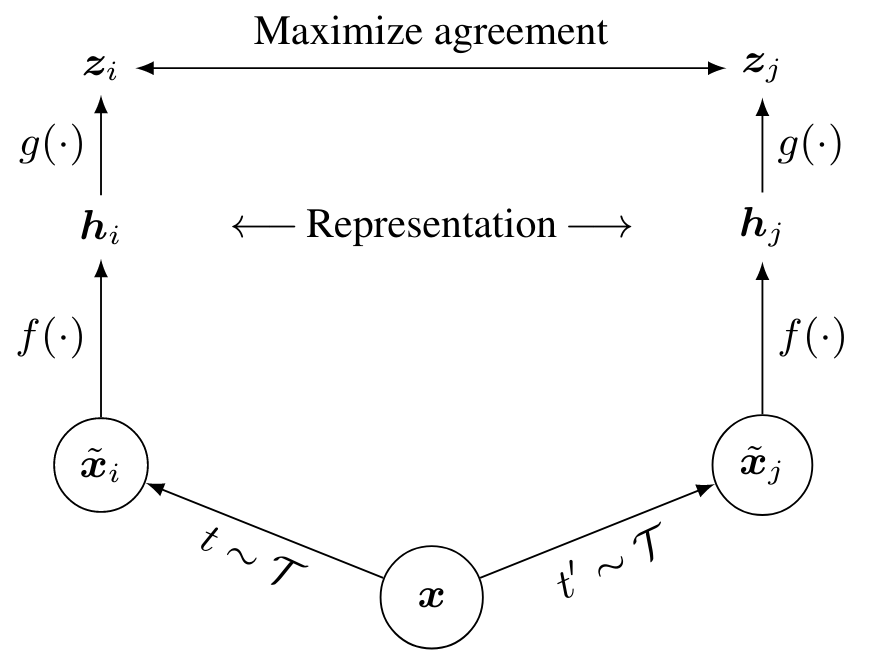
\includegraphics[width = 200pt]{simclr.png}
  \caption{Visualizing the representations and the projection heads. Figure from the SimCLR paper~\cite{DBLP:journals/corr/abs-2002-05709} i}
\end{figure}

\noindent The contrastive loss wants to maximize the mutual agreement of two views of the same image. 
The loss function is called NT-Xent (normalized temperature-scaled cross entropy loss) and is defined as following:

\begin{equation}
    \ell_{i,j} = -\log \frac{\exp(\mathrm{sim}(\tilde{x}_i, \tilde{x}_j)/\tau)}{\sum_{k=1}^{2N} \mathds{1}_{k \neq i} \exp(\mathrm{sim}(\tilde{x}_i, \tilde{x}_j)/\tau}
\end{equation}
where $\tau$ is the temperature parameter and $\mathrm{sim}(x_i, x_j)$ is the cosine similarity between $x_i$ and $x_j$.

\noindent In representation learning there are positive and negative pairs. Consider a batch of size $N$: \\
For each image in this batch stochastic data augmentation is applied twice resulting in a new batch of size $2N$. 
Positive pairs are now those $\tilde x_i$ and $\tilde x_j$ that were originally from the same image before data augmentation. The other $2N-2$ augmented images are considered negative examples. The contrastive loss is then calculated to all positive pairs $(i,j)$ and $(j,i)$ and
the resulting gradient is applied to the parameters of the encoder.

\begin{algorithm}[h]
\begin{algorithmic}[1]
\caption{SimCLR Pseudocode, taken from SimCLR paper~\cite{DBLP:journals/corr/abs-2002-05709}}
    \State \textbf{input:} batch size $N$, constant $\tau$, structure of $f$, $g$, $\mathcal{T}$.
    \For{sampled minibatch $\{\bm x_k\}_{k=1}^N$}
    \State \textbf{for all} $k\in \{1, \ldots, N\}$ \textbf{do}
        \State $~~~~$draw two augmentation functions $t \!\sim\! \mathcal{T}$, $t' \!\sim\! \mathcal{T}$
        \State $~~~~$\textcolor{gray}{\# the first augmentation} 
        \State $~~~~$$\tilde{\bm x}_{2k-1} = t(\bm x_k)$
        \State $~~~~$$\bm h_{2k-1} = f(\tilde{\bm x}_{2k-1})$  \textcolor{gray}{~~~~~~~~~~~~~~~~~~~~~~~~~~~~~~\# representation}
        \State $~~~~$$\bm z_{2k-1} = g({\bm h}_{2k-1})$  \textcolor{gray}{~~~~~~~~~~~~~~~~~~~~~~~~~~~~~~~~~~~~\# projection}
        \State $~~~~$\textcolor{gray}{\# the second augmentation} 
        \State $~~~~$$\tilde{\bm x}_{2k} = t'(\bm x_k)$
        \State $~~~~$$\bm h_{2k} = f(\tilde{\bm x}_{2k})$      \textcolor{gray}{~~~~~~~~~~~~~~~~~~~~~~~~~~~~~~~~~~~~\# representation}
        \State $~~~~$$\bm z_{2k} = g({\bm h}_{2k})$      \textcolor{gray}{~~~~~~~~~~~~~~~~~~~~~~~~~~~~~~~~~~~~~~~~~~\# projection}
    \State \textbf{end for}
    \State \textbf{for all} $i\in\{1, \ldots, 2N\}$ and $j\in\{1, \dots, 2N\}$ \textbf{do}
    \State $~~~~$ $s_{i,j} = \bm z_i^\top \bm z_j / (\lVert\bm z_i\rVert \lVert\bm z_j\rVert)$ \textcolor{gray}{~~~~~~~~~~~~~~~~~~\# pairwise similarity}
    \State \textbf{end for}
    \State \textbf{define} $\ell(i, j)$ \textbf{as}~ $\ell(i, j) \!=\! -\log \frac{\exp(s_{i,j}/\tau)}{\sum_{k=1}^{2N} \mathds{1}_{k \neq i}\exp(s_{i, k}/\tau)}$
    \State $\mathcal{L} = \frac{1}{2N} \sum_{k=1}^N \left[ \ell(2k\!-\!1, 2k) + \ell(2k, 2k\!-\!1)\right]$
    \State update networks $f$ and $g$ to minimize $\mathcal{L}$
    \EndFor
    \State \textbf{return} encoder network $f(\cdot)$, and throw away $g(\cdot)$
\end{algorithmic}
\end{algorithm}


\section{Reinforcement Learning}
Reinforcement learning differs from other types of machine learning because usually the dataset is not a static one.
It is dynamically created by interacting with an environment over time. The environment has
a state space $S$, an action space $A$ containing all valid actions, 
a reward function $R : S\times A \xrightarrow{} \mathbb{R}$ and a
dynamics function $p : S\times A\times S \xrightarrow{} \mathbb{R}$. Data collected
in this fashion is often refereed to as trajectory. The reward function gives indication 
whether progress towards the desired goal has been made.\\
A so-called agent choose actions $a \in A$, given a state $s \in S$ as the input. The environment then returns the next state $s' \in S$ and a scalar, which is called the reward. The part of the agent that is responsible for action selection is called the policy model $\pi : S \xrightarrow{} A$.
The probability of transitioning from state $s$ to the next state $s'$ by performing action $a$ is described by the environment dynamics function $p(s, a, s')$~\cite{Sutton1998}.\\
Maximizing the reward signal over time is the goal of RL-agents. The next state is directly depended on the
selected action. A timestep $t$ contains the tuple $(state, action, reward, done)$. Done is an indicator
whether $t$ is the last step of an episode. This means that the next state is the terminal state such as the a checkmate
in a game of chess. A trajectory contains $T$ timesteps.
State, action, reward and done signal experienced at timestep $t$ are denoted by the tuple $(s_t, a_t, R_{t+1}, d_t)$.\\
An agent interacting with its environment is often formalized as a Markov decision process because the assumption of Markov property is very useful.
Markov property means that the next state $s_{t+1}$ only depends on the current state $s_t$. 
In terms of conditional
probabilities that means that $\text{prob}(s_{t+1}|s_t) = \text{prob}(s_{t+1}|s_t,s_{t-1},...,s_0)$.
A theoretical framework as well as domain knowledge for crafting efficient states can be derived
from this formalization.

\begin{figure}[h]
  \centering
  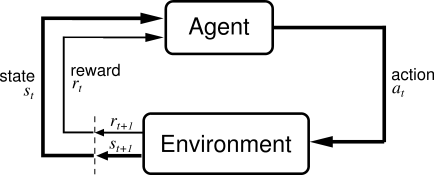
\includegraphics[width = 200pt]{agent_env.png}
  \caption{A visualization from the Sutton and Barto Book~\cite{Sutton1998}}
\end{figure}

\noindent The rewards signal replace the labels used in supervised learning as they are
combined to form such targets in a variety of ways. A discount factor $\gamma \in [0,1]$ is introduced that
balances receiving immediate rewards against prioritizing long term rewards. Going closer towards 0 means
that immediate rewards gain high priority while the opposite is true when approaching 1.\\
The expected return at step $t$ is called $G_t$ and is an approximation of the discounted
expected rewards when starting in state $s_t$ and following policy $\pi$.
There are different ways of calculating an expected return, most notably Temporal Difference (TD) and Monte Carlo estimation~\cite{Sutton1998}.\\
Monte Carlo (MC) estimation defines $G_t$ as the discounted sum of all rewards received after time $t$.
\begin{equation}
    G_t^{MC} = \sum_{i=t}^T \gamma^{i-t} R_{i+1}
\end{equation}
This is an unbiased sample, but calculating our expected return this way leads to a
high variance of estimates.
TD($n$) methods are taking the next $n$ received rewards after step $t$ and then 
bootstrap a value. To bootstrap
the value of a state we introduce a state-value function $v_\pi : S \xrightarrow{} \mathbb{R}$, which
is an estimate of the discounted sum of rewards when starting in $s_t$.

\begin{equation}
    G_t^{TD(n)} = \gamma^n v_\pi(s_{t+n}) + \sum_{i=t}^{t+n} \gamma^{i-t} R_{i+1}  
\end{equation}

\noindent TD($\infty$) is equal to the Monte Carlo return because the entire trajectory is summed and
the value of the terminal state is 0 by definition.
Choosing a low value for $n$ will decrease variance, but increase bias and the other way around.
This is knows as the bias-variance tradeoff.\\
If the state-value function is a neural network, it is trained on the mean squared error between
its prediction of the state-value $v_\pi(s)$ and the expected return $G_t$. If we are using a TD($n$) method the target
value is dependant on $v_\pi$, but the gradient w.r.t. the parameters of $v_\pi$ is not calculated through the target $G_t$. 
These methods are sometimes called semi-gradient methods~\cite{Sutton1998} and
no guarantee of convergence can be expected for a moving target.
There are workarounds to increase stability such as using a secondary model to predict
the target value and periodically copying over the weights~\cite{hessel2017rainbow}.\\

\noindent The algorithm which is chosen as the agent can be
separated into two major categories: On-policy and off-policy. On-policy algorithms need
to be trained on trajectories which are collected by following its policy $\pi$. Most on-policy
models use a variaton of a policy gradient method~\cite{NIPS1999_464d828b} as update rule. The policys parameters are updated
with respect to maximizing their expected return. Sometimes a factor to weight different trajectories by their respective policys probabilities
is used, the importance sampling ratio $r$. For two policies $\pi$ and $b$ the importance sampling ratio is defined as:
\begin{equation}
    r : S\times A \xrightarrow{} \mathbb{R}
\end{equation}
\begin{equation*}
    r(s, a) = \frac{\pi(a|s)}{b(a|s)}
\end{equation*}
If appropriate for the selected agent this allows us to train on data obtained by other policies. The data for
on-policy models can also only be used once for training, because after taking a gradient step the distribution $\pi(\cdot|s)$ changes
and therefore the data is no longer generated by our new $\pi$.\\
Off-policy algorithms on the other hand can naturally be optimized
by data collected from any policy. Often this is true because off-policy methods use 
action-value functions $q_\pi : S\times A \xrightarrow{} \mathbb{R}$, 
instead of state-value functions. 
That means that in contrast to the state-value function the action-value function $q_\pi$
computes the expected return given state and action.
We can represent $v_\pi$ in term of $q_\pi$.
In discrete action spaces $v_\pi(s_t) = \sum_a \pi(a|s_t)
q_\pi(s_t, a)$, while in continuous action spaces the sum would be replaced by an integral over $a$.
The policy is then to simply select the action with the highest action-value. This approach is called greedy.
If a random action is selected at probability $\epsilon$ instead, we call the method epsilon-greedy.\\
Each of the two types of policies have their advantages. Off-policy is a lot better in terms of
sample efficiency since data can not only be reused, but also data collected from other policies can be used.
On-policy on the other hand usually learns a stochastic policy $\pi(\cdot|s) > 0$ which means that it keeps
selecting different actions and therefore explore more.\\
The act of selecting sub-optimal actions in order to find a more rewarding path to the goal is called exploration.
Taking the way that yielded the most reward in the past is called exploitation. These two create another
important tradeoff in RL, the exploration exploitation tradeoff. A policy will need to explore
sufficiently well before it keeps exploiting or it may never find the optimal trajectory. Optimal here means
the most reward collected.

\subsection{Arcade Learning Environment and Ms. Pac-Man}

The Arcade Learning Environment~\cite{DBLP:journals/corr/abs-1207-4708} has proven itself
as a good benchmark for RL agents. It withstood the test of time and is the de facto standard
for evaluating performance~\cite{DBLP:journals/corr/abs-1709-06009}. Best practices 
for using it include gray scaling the frames and stack 4 of them because some blinking
elements can only be seen if the environment is observed for this time. It is also
very common to rescale the frames to $84\times 84$, resulting in a state space consisting of $S = \{0,...,255\}^{4\times 84\times 84}$.
The full action space consists of 18 different action $A =\{0,...,17\}$, where only a single action
can be selected for each timestep $t$.\\
\begin{figure}[h]
    \centering
    \subfloat[Beginning of an episode]{{
\includegraphics[width=4cm]{pacman_start.png} }}
    \qquad
    \subfloat[After 500 frames have passed]{{
\includegraphics[width=4cm]{pacman.png} }}
    \caption{Two different frames of the game Ms. Pac-Man}
\end{figure}

\noindent Of the over 50 games contained in the ALE we will take a closer look at the environment Ms. Pac-Man.
The player controls his character through a grid with walls and loses a life if a ghost
touches him. A player has three life in totals before we consider an episode to have ended.
In Ms. Pac-Man the player can obtain by rewards by collection dots and fruits on the map. Alternatively
an energy pill can be collected and ghosts can be killed for large rewards.\\
This leads to a challenging environment which can be tackled with a variety of different
plans e.g. prioritizing the collection of an energy pill and killing as many ghosts as possible
while largely neglecting the collection of rewards for picking up dots.


\section{Trust Region Optimization Methods}

Trust Region Policy Optimization~\cite{pmlr-v37-schulman15} was first introduced by Schulman et al.
and aims to improve stability of training by limiting the Kullback–Leibler divergence $D_{KL}(\pi_\theta|\pi_{\theta_{\text{old}}})$
between the new policy $\pi_\theta$ and the old policy $\pi_{\theta_{\text{old}}}$. The KL divergence is a measure of how different
one distribution $\pi_{\theta_{\text{old}}}(\cdot|s)$ is from another distribution $\pi_\theta(\cdot|s)$.\\

\noindent This is achieved in~\cite{pmlr-v37-schulman15} by computing the second order derivative and adding 
a hard constraint to the weight update. 
\begin{equation}
    \theta_{\text{next}} \xleftarrow{} \arg \max_{\theta} {\mathcal L}_{\text{TRPO}}(s, a) 
\end{equation}
\begin{equation*}
    \text{s.t.} \; {D}_{KL}(\pi_\theta|\pi_{\theta_{\text{old}}}) \leq \delta
\end{equation*}

\noindent where $\delta$ is the maximum KL divergence and ${\mathcal L}_{\text{TRPO}}$ is called surrogate 
advantage. ${\mathcal L}_{\text{TRPO}}$ is the estimated advantage weighted by the importance
sampling ratio between the new and the old policy. We define the importance sampling ratio between
the new policy $\pi_\theta$ and the old policy $\pi_{\theta_\text{old}}$ as:
\begin{equation}
    r : S \times A \xrightarrow{} \mathbb{R} 
\end{equation}
\begin{equation*}
    r(s, a) = \frac{\pi_{\theta}(a|s)}{\pi_{\theta_{\text{old}}}(a|s)}
\end{equation*}
where $s \sim S$ is one state drawn from the set of all states and $a \sim A$ is a
valid action selected from the set of all actions.

\noindent Our estimate for the advantage function $\hat A(s_t, a_t)$ at time step $t$ is
calculated via generalized advantage estimation~\cite{Schulmanetal_ICLR2016} (GAE). Here $\lambda$ is
the factor which controls the bias-variance tradeoff. A value near zero has typically a lot
less variance, but high bias. For a value near one it is the other way around.
Building a return this way is more flexible than using a n-step return method~\cite{DBLP:journals/corr/abs-2006-05990}.

\begin{equation}
    \hat A_\pi : S \times A \xrightarrow{} \mathbb{R} 
\end{equation}
\begin{equation*}
    \hat A_\pi(s_t, a_t)  = R_{t+1} + \gamma v_\pi(s_{t+1}) - v_\pi(s) + (1-d_t) \lambda \gamma \hat A_\pi(s_{t+1}, a_{t+1})
\end{equation*}

where $d_t \in \{0,1\}$ is an indicator whether time step $t$ was the last of an episode.
$v_\pi$ is the value function or critic of the algorithm.
The advantage function depends on the policy it is calculated for, so a subscript
indicates for which policy it is generated.

\begin{equation}
    {\mathcal L}_{\text{TRPO}}: S \times A \xrightarrow{} \mathbb{R}
\end{equation}
\begin{equation*}
    {\mathcal L}_{\text{TRPO}}(s, a) ={r(s, a) \hat A_{\pi_{\theta_{\text{old}}}}(s,a)}
\end{equation*}

\noindent This method stabilizes training but at the cost of computing the second order derivative
which requires a lot of compute.\\
To combat the additional required compute more modern trust region optimization methods
replace the hard constraint with a penalty term or clip the step size in some other way.

\subsection{Proximal Policy Optimization}
\noindent Proximal Policy Optimization~\cite{DBLP:journals/corr/SchulmanWDRK17} or PPO was first
introduced by OpenAI in 2017 and
has been a very popular on-policy algorithm which supports both continuous and
discrete action spaces. OpenAI also emphasised that it has become their default
reinforcement learning algorithm due to its ease of use and good performance.\\
There are a few different loss terms shown in the paper, but I will focus on the main
suggestions, the PPO-Clip as it outperforms all other methods that use KL divergence penalty terms~\cite{DBLP:journals/corr/abs-2006-05990}.
The main idea behind PPO is to limit the step size as to avoid performance
collapse. To do so, one chooses an $\epsilon \in [0,1]$ as the policy clip ratio,
which is the maximal divergence from the old policy. This clipping is achieved
by construction the loss in such a way that the gradient for a divergence greater than $\epsilon$ is zero.
We use the same importance sampling ratio between the new policy and the old one.
PPO updates its policy parameters $\theta$ via gradient ascent on the surrogate objective ${\mathcal L}_{\mathrm{CLIP}}$:

\begin{equation}
    {\mathcal L}_{\mathrm{CLIP}}: S\times A \xrightarrow{} \mathbb{R}
\end{equation}
\begin{equation*}
    {\mathcal L}_{\mathrm{CLIP}}(s, a) = \mathrm{min}(r(s,a) \hat{A}_{\pi_\theta}(s,a), \mathrm{clip}(r(s,a), 1 - \epsilon, 1 + \epsilon)\hat{A}_{\pi_\theta}(s,a))
\end{equation*}
\noindent An entropy term of the distribution $\pi_\theta(\cdot|s)$ can be added
to the loss term in order to encourage more exploration and a stochastic policy.

\begin{figure}[h]
    \centering
    \subfloat[$\hat A > 0$]{{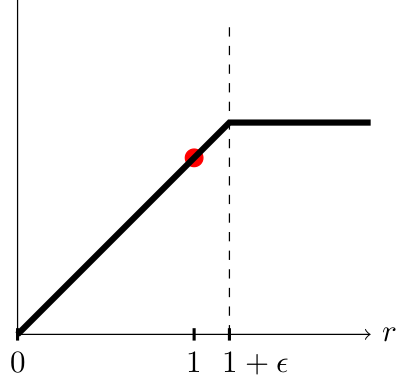
\includegraphics[width=4cm]{a_big_0.png} }}
    \qquad
    \subfloat[$\hat A \leq 0$]{{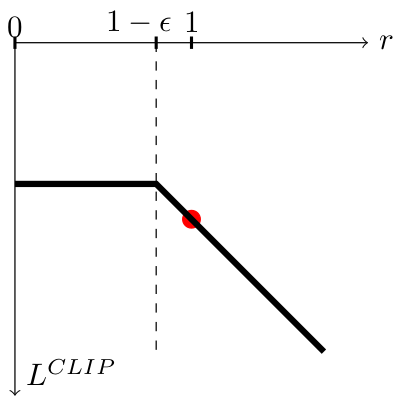
\includegraphics[width=4cm]{a_smal_0.png} }}
    \caption{Figure from original PPO paper visualizing the clipped objective~\cite{DBLP:journals/corr/SchulmanWDRK17}}
\end{figure}

\noindent Figure 6. shows the effect of the clipped objective. Once the ratio
$r$ get bigger than the threshold $\epsilon$, the objective function get clipped and the gradient
beyond that point becomes zero. It is uncapped if the advantage is negative
and $r$ is positive because this means the negative advantage was scaled big because 
the selected, bad action became a lot more probable.\\
With this objective we obtain most of the benefits from TRPO but do not have
to compute the second order derivative.

\noindent The policy $\pi : S \xrightarrow{} A$ is represented by a neural network, which uses
the architecture of the original DQN-Paper~\cite{DBLP:journals/corr/MnihKSGAWR13}, consisting of
a convolution layer, which uses 16 filters of size 8 x 8 and stride 4,
followed by another, with 32 filter of size 4 x 4 with stride 2. The feature maps are then
flattened and transformed through a fully connected layer with 256 weight units.
The output layer is a fully connected layer as well and has one unit for every
action of the action space $A$ and is followed by the softmax function. 
An action is selected by sampling from this distribution and passed to environment.\\
To simplify notation we drop the $\theta$ when indexing policies, so $\pi$ refers to $\pi_\theta$ and
$\pi_{old}$ refers to the old policy $\pi_{\theta_{old}}$.
Trajectories generated by this network are used once for updating the policys
parameters before they are thrown out. At the time the trajectory is generated,
the probability of the selected action is saved and serves as the value for
$\pi_{old}(a|s)$ in the importance sampling ratio $r(s,a)$.\\
The value function $v_{\pi_\theta}(s_t)$ is also represented by a neural network and
is trained on the expected return $G_t = v_{\pi_{old}}(s_t) + \hat A_\pi(s_t,a_t)$
via mean squared error to the predicted value $\hat y = v_\pi(s_t)$. 
While the value function predicts the values if following the policy $\pi$, which is
indicated by the subscript, it has its own set of parameters $\psi$, which are updated
via gradient descent on its loss function $\mathcal{L}_{value}$.

\begin{equation}
    \mathcal{L}_{value}(\hat y, G_t) = MSE(\hat y, G_t)
\end{equation}

\noindent A PPO training phase, or policy phase consists of performing gradient steps to maximize $\mathcal{L}_{CLIP}$
on all collected trajectory data and a critic training phase to minimize $\mathcal{L}_{value}$.
The critic and the policy network can share some layers, in
which case the value part is an additional neuron in the output layer
which acts as state-value estimate. A benefit of this is that both,
the value loss function and the surrogate objective, may learn representations which are mutual
beneficial for the tasks of each other are learned. The disadvantage of this is interference between
the two tasks.

\subsection{Phasic Policy Gradient}

Phasic Policy Gradient (PPG)~\cite{DBLP:journals/corr/abs-2009-04416} aims to the improve the
sample efficiency of PPO and get the best of both world from the shared-or-separate network
dynamic. This is achieved by using a shared-network architecture for the policy and an independent
critic network. This means that our policy has one more output neuron than there are valid actions.
This output neuron will be referred to as the value head $\pi_{aux}$. All other output neurons are still
considered to be a distribution over the action space, which mean that they are output by $\pi(a|s)$.\\

\begin{figure}[h]
  \centering
  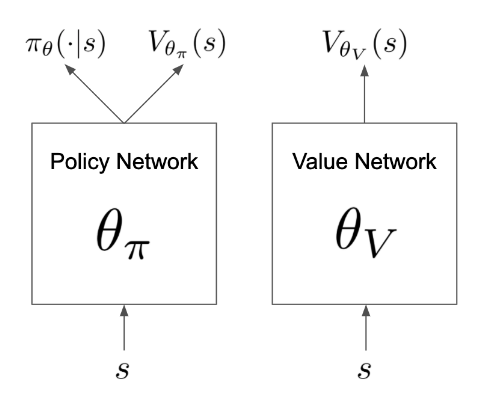
\includegraphics[width = 150pt]{ppg_heads.png}
  \caption{Left the two heads of the policy network $\pi$ and right the independent critic. This thesis refers to the policys value head as $\pi_{aux}$ instead of $V_{\theta_\pi}$. Figure from the original PPG paper~\cite{DBLP:journals/corr/abs-2009-04416}}
\end{figure}

\noindent In a new training phase, which is called the auxiliary phase, this extra value head is trained via
a combination of the value loss $\mathcal{L}_{value}$ and a behavior cloning loss. This loss limits divergence from the
old policy, while improving value estimation. The hyperparameter $\beta_{clone}$ controls
the size of the behavior cloning loss term and is set to 1. The auxiliary loss is then
computed for $\hat y = \pi_{aux}(s_t)$ and $G_t = \pi_{aux}(s_t) + \hat A_\pi(s_t,a_t)$. 
The advantage function $\hat A_\pi$ in $G_t$ is also dependent on the output 
value of the auxiliary head $\pi_{aux}$ and not on the critic $v_\pi(s)$.

\begin{equation}
    \mathcal{L}_{aux}(\hat y, G_t) = \mathcal{L}_{value}(\hat y, G_t) + \beta_{clone}D_{KL}(\pi|\pi_{\text{old}}))]
\end{equation}

\noindent In auxiliary phases the critic is also trained and updates its parameters $\psi$, but has no influence on the policy networks weights.
These phases work best if not performed too frequently as to not disturb
the policy learning. The authors recommended to do 3 auxiliary epochs every 32 policy epochs.

\begin{figure}[h]
  \centering
  \includesvg[width = 250pt]{ppg.svg}
  \caption{PPG for 4 stacked Atari frames. The policy network $\pi_\theta$ with the extra value head in the output layer results in 19 total output neurons.}
\end{figure}

\noindent Sometimes the value loss get scaled down or the maximum divergence from
the old policy is clipped via an approximation of the KL divergence. Due to auxiliary epochs being performed
infrequently this does not hurt runtime in a meaningful way.\\

\begin{algorithm}[H]
\begin{algorithmic}[1]
\caption{PPG Pseudocode}
\For{phase = 1,2,...}
    \State Initialize empty buffer B
    \For{iteration = 1,2,..., N}
        \State Perform rollouts under current policy $\pi$
        \State Compute value function target $v_\pi(s)$
        \For{epoch = 1,2,...,$E_\pi$}
            \State Optimize $\mathcal{L}_{CLIP}$ w.r.t. the policys parameters $\theta$
        \EndFor
        \For{epoch = 1,2,...,$E_V$}
            \State Optimize $\mathcal{L}_{value}$ w.r.t. the critics parameters $\psi$
        \EndFor
        \State Add all $s_t, v_\pi(s)$ to B
        \State Compute and store current policy $\pi_{old}$ for all states $s_t$ in B
        \For{epoch = 1,2,...,$E_{aux}$}
            \State Optimize $\mathcal{L}_{aux}$ w.r.t. $\theta$ on all data in B
            \State Optimize $\mathcal{L}_{value}$ w.r.t. $\psi$ on all data in B
        \EndFor
    \EndFor
\EndFor
\end{algorithmic}
\end{algorithm}

\noindent The algorithm as described in the PPG paper~\cite{DBLP:journals/corr/abs-2009-04416}. $E_\pi$ is the number of 
epoch the policy is trained on the data it generated. $E_V$ is the number of epochs the critic is 
trained on the collected data and $E_{aux}$ is the number of times auxiliary epochs are executed.

\section{Active Pre-Training}

Active Pre-Training (APT)~\cite{DBLP:journals/corr/abs-2103-04551} is a method that combines self-supervised
and reinforcement learning. APT aims to create an objective in a reward free environment and use it to pre-train
the agent. The goal is to learn representations and behaviors which are useful for various tasks.
Goals are communicated to the agent after the pre-training phase by defining a reward function and
exposing these task-specific rewards to the agent. This helps as a starting point for learning new
tasks~\cite{DBLP:journals/corr/abs-2106-09226}. Tasks which are defined after pre-training are usually
called downstream tasks.\\
The reward function of the environment is replaced during the pre-training by a function
which computes the entropy in an abstract representation space. This entropy is then used as the reward
which the agent maximizes and explores the environment. APT uses
SimCLR~\cite{DBLP:journals/corr/abs-2002-05709} to learn the representations that are used
to calculate the entropy reward.\\
When transitioning from state $s_t$ to the next state $s_{t+1}$,
the next state are encoded by a neural network $f : S \xrightarrow{} \mathbb{R}^n$ where $n$ is much small than 
the dimension of $S$. We will refer to this representation as $z_t$.
The neural network used for this contains a convolution layer with 32 filters of size 8 and stride 4, followed by
another convolution layer with 64 filters of size 4 and stride 2. The final convolution layer has also 64 filters, but of
size 3 and stride 1. An Exponential Linear Unit (ELU) is used as the activation function between the layers.
After the convolution layers a fully connected layer is applied as the output layer, which is followed by 
a LayerNorm and a Tanh activation function. The authors mention it helps to use spectral normalization for the 
convolution layers~\cite{DBLP:journals/corr/abs-2103-04551}.\\
The projection head $g$, which takes the output from the encoder $z_t$ as input, consists of a two layer MLP, using ELU between them.
This projection is used to update the encoder with the NT-Xent loss and with labels derived as described in SimCLR.\\
The learned representation $z_{t}$ is used to form a reward for the transition. The main idea
is to measure the average distance between each data point and its k nearest neighbors~\cite{doi:10.1080/01966324.2003.10737616}.
The applied data augmentations are a a simple change in brightness and cropping of the original frames
after applying a replication padding of size 4 to it. By applying only soft data augmentations
we make sure that the semantic meaning of the image is not changed. For example if rotation
is be used the meaning of the action to go right or left changes. Those carefully selected
data augmentations are from Data Regularized Q~\cite{DBLP:journals/corr/abs-2004-13649}.

\begin{equation}
    H_{\text{particle}}: Z\times Z \xrightarrow{} \mathbb{R}
\end{equation}
\begin{equation*}
    H_{\text{particle}}(z) = \sum_{i=1}^n \text{log}(c + \frac{1}{k} \sum_{z_j \in N_k(z_i)} ||z_i - z_j||)
\end{equation*}
where $N_k$ denotes the $k$ nearest neighbors of $z_i$ and $c$ is a constant for numerical stability, fixed to 1.
This $H_{\text{particle}} $ is proportional to the particle-based entropy
estimation suggested in earlier works~\cite{DBLP:journals/corr/abs-2103-04551}.
During the pre-training this approximation of the particle based entropy acts as the
reward function for any encountered transition. This is done by computing the $k$ nearest
neighbors in a batch. Therefore this method therefore profits from larger batch sizes. For a
singular transition the reward if defined in relation to its batch by:

\begin{equation}
    R(s_t, a_t, s_{t+1}) = \text{log}(c + \frac{1}{k} \sum_{z_j \in N_k(f(s_t))} ||f(s_t) - z_j||)
\end{equation}
where $z_j$ are the representations of the next states within a batch, which are considered as the particles.
The rewards are normalized by dividing them by a running estimate of the mean to keep them on a consistent scale. 

\begin{figure}[h]
    \centering
    \subfloat{{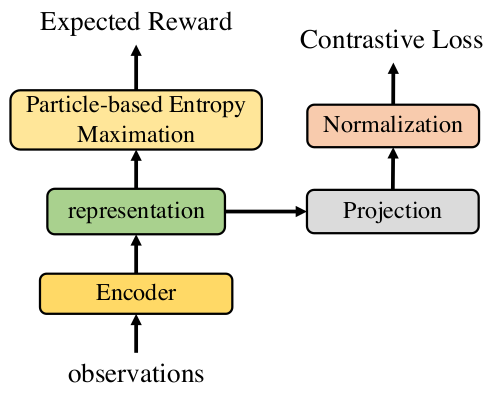
\includegraphics[width=5cm]{apt_graph.png} }}
    \qquad
    \subfloat{{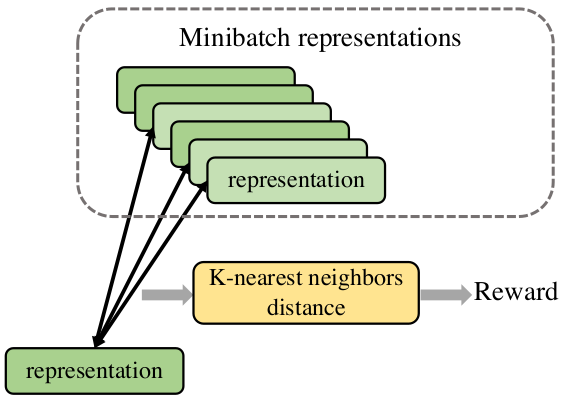
\includegraphics[width=5cm]{repr_graph.png} }}
    \caption{Figures from the APT paper~\cite{DBLP:journals/corr/abs-2103-04551} visualizing the procedure of 
    generating rewards and learning representations. Observation is a synonym for a state which might not be
    fully observable.}
\end{figure}

\noindent A training phase of APT starts with receiving a state from the environment and then selecting an action
according to an off-policy algorithm. 
The agent then performs this action in its environment and goes to the next state.
This transition tuple $(s_t, a_t, s_{t+1})$ is then saved to the replay buffer.
A minibatch is then sampled from this replay buffer and the encoder is then trained on it with the SimCLR objective.
Actions are then selected according to $\pi$ and the action-value function $q_\pi$ is trained. 
The reward in the expected return is computed via the self-supervised reward function $R$.\\

\begin{algorithm}[h]
\begin{algorithmic}[1]
\caption{APT Pseudocode}
\State Randomly initialize encoder $f$
\State Randomly initialize policy $\pi$ and action-value function $q$
\For{phase = 1,2,...}
    \For{t = 1,2,..., T}
        \State Receive state $s_t$ from the environment
        \State Take action $a_t \sim \pi(\cdot|s_t)$, receive next state $s'_t$
        \State Ignore the reward $R_{t+1}$ from the environment
        \State $D \gets D \cup (s_t, a_t, s'_t)$
        \State Sample minibatch from $D$ and train neural encoder on it
        \For{i = 1,2,...,N}
            \State Sample action ${a'}_i \sin \pi(\cdot|s'_i)$
            \State $\hat Q_i = Q(s'_i, a'_i)$
            \State Compute particle-based entropy reward $R_i$
            \State $y_i \gets R_i + \gamma \hat Q_i$
        \EndFor
        \State $\text{loss}_q = \sum_i (q(s_i, a_i) - y_i)^2$
        \State Gradient descent step on $q$ and $\pi$
    \EndFor
\EndFor
\end{algorithmic}
\end{algorithm}

\noindent The off-policy algorithm Dr.Q~\cite{DBLP:journals/corr/abs-2004-13649} uses an epsilon-greedy
policy to select actions. For a probability of epsilon
a random action is selected instead of the one with the highest action-value.
The replay buffer $D$ is the dataset which contains all collected experience.

\section{APT with Phasic Policy Gradient}
The general application of APT is to pre-train a policy in a given environment and adapt it
to downstream tasks afterwards. This means that there are multiple, similar tasks e.g.
the environment of a robot that picks and places warehouse items. Another possibility is
that the task has a very sparse reward function. APT helps to explore the state space beforehand
and helps thereby performs especially for sparse reward taks~\cite{DBLP:journals/corr/abs-2103-04551}.
Because of this and the fact that the pre-training of APT requires 250 million steps 
APT may be useful for on-policy algorithms too. Although they cannot compete
with off-policy algorithms in terms of sample-efficiency they require less computational
power on average to learn a successful policy. 
This is the motivation behind the idea of combining PPG with APT.\\

\noindent Replacing the action-value function $q_\pi$ with the state-value function $v_\pi$ and the expected return TD(1)
with the GAE~\cite{Schulmanetal_ICLR2016} return allows to train the critic in the same manner APT trains the action-value function.\\
The policy $\pi$ is trained on the PPO objective $\mathcal{L}_{CLIP}$ with the advantages computed by GAE
and the state-value function of the critic.
Auxiliary epochs train the auxiliary value head $\pi_{aux}$ and the critic on their respective objectives.\\
Opposed to the off-policy training PPG collects a certain number of timesteps and trains 
once on them before throwing them away. The number of collected timesteps 
should not be too large. When we iterate through the data and update the model
after each batch the policy should still very similar to the policy that produced the
data. Elsewise the data is not really on-policy anymore.
On the other hand the training of the encoder with on the 
SimCLR objective benefits from larger batch sizes.
The particle-based entropy also depends on sufficiently large batch sizes so that it is more consistent.
Finding a middle ground between these objectives seems to work best with a batch size and rollout length of 512.

\subsection{Parallelism-Variance Dilemma}
To shorten computation time by reducing the required amount of sequential computations 
16 parallel environments are used to collect the data.
Two separate buffers are created, one for the policy, critic and auxiliary training of size 512
and one for the training of the encoder of size 10000. It is important to select a large size for the encoder buffer
because the states generated from the 16 environments are all sampled from the same policy. 
This can lead to a counterproductive behavior in the SimCLR objective, especially at the beginning
of training, when the buffer is not yet full.
States which are very close in state space are then treated as negative examples and pushed away from each other. 
States can be very close to each other when their frames are all the beginning of an episode or
if the same action is always selected and the agent always moves to the same wall.
While those states are pushed away from each other, they actually are
so similar they should be grouped together in representation space.
This problem will be referred to as the Parallelism-Variance Dilemma.
 
\begin{figure}[h]
  \centering
  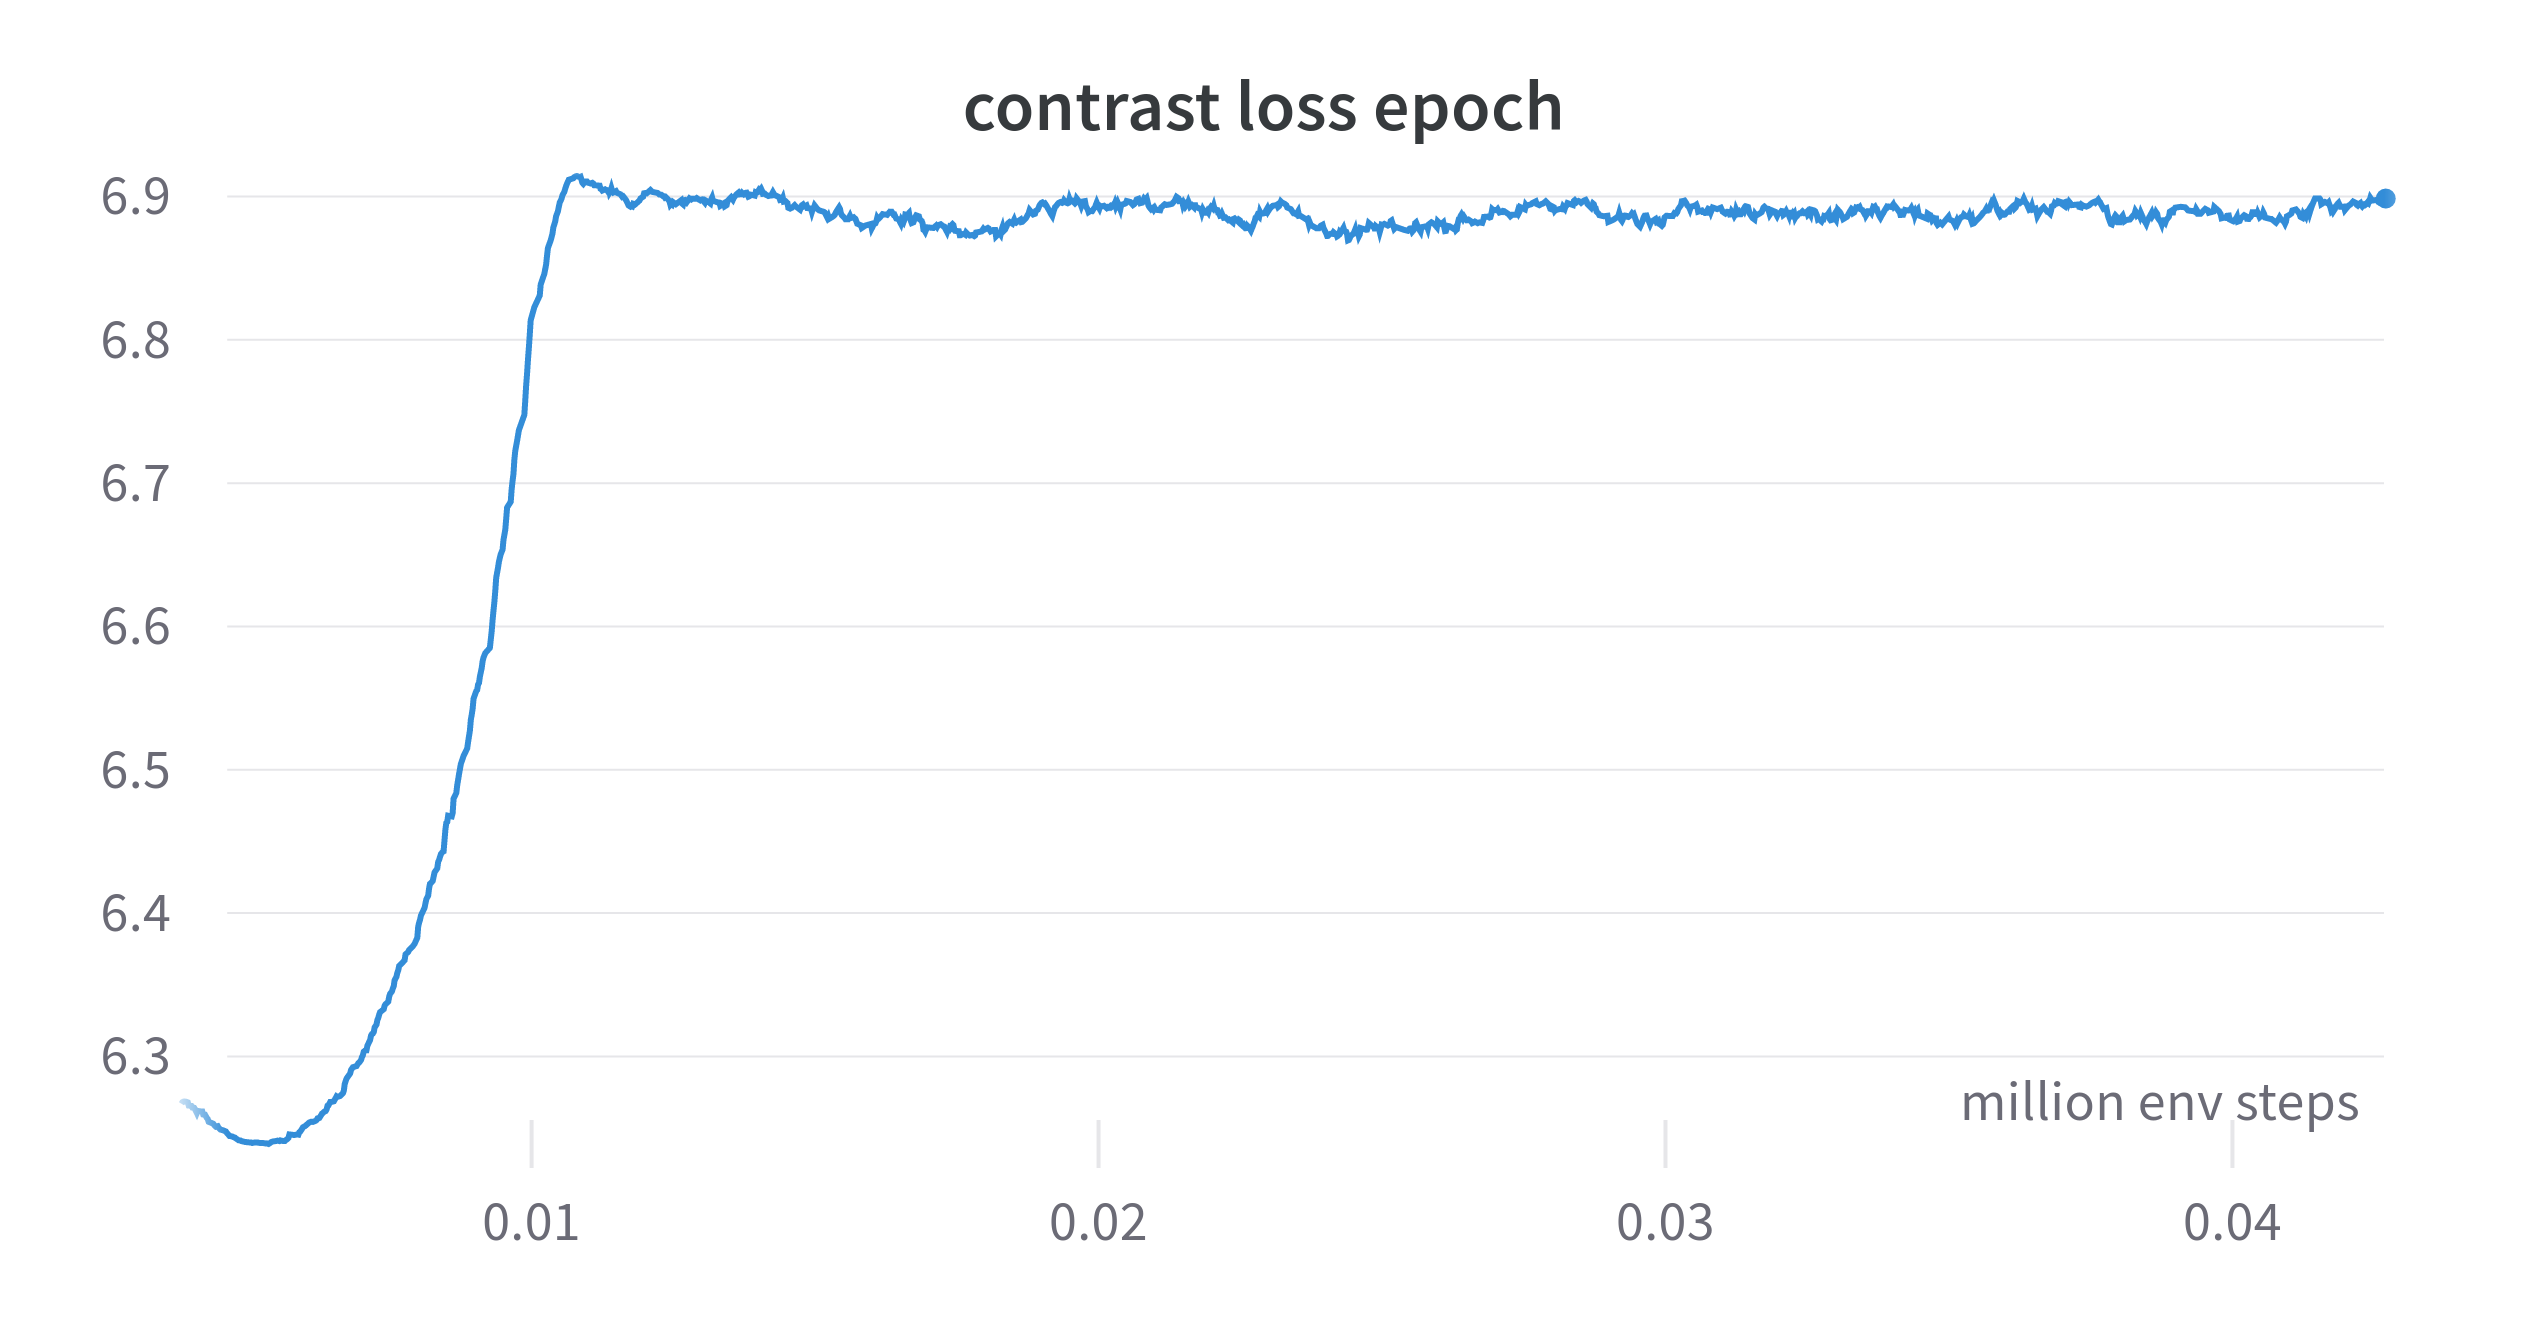
\includegraphics[width = 250pt]{contrast_loss.png}
  \caption{Contrastive loss increases in the beginning of training due too low variance of the states. All plots
  are created with WandB~\cite{wandb}.}
\end{figure}

\noindent This interference disrupts the encoder training and limits the amount of
parallel environments and thus the parallelism.

\noindent A key moment of the combination of PPG with APT is when the contrastive loss drops and
the encoder outputs better representations. This dramatically increases the amount of rewards the agent
collects and too large gradient steps are taken, leading to single action selection policy collapse. A vicious spiral of events is thereby triggered.
Since all actions performed in all environments are the same, all collected states
will be very similar. The buffer of the encoder becomes filled with states that are 
very close to each other, but the NT-Xent objective tries to push them away.
This leads to a loop of the Parallelism-Variance Dilemma. 
\begin{figure}[h]
  \centering
  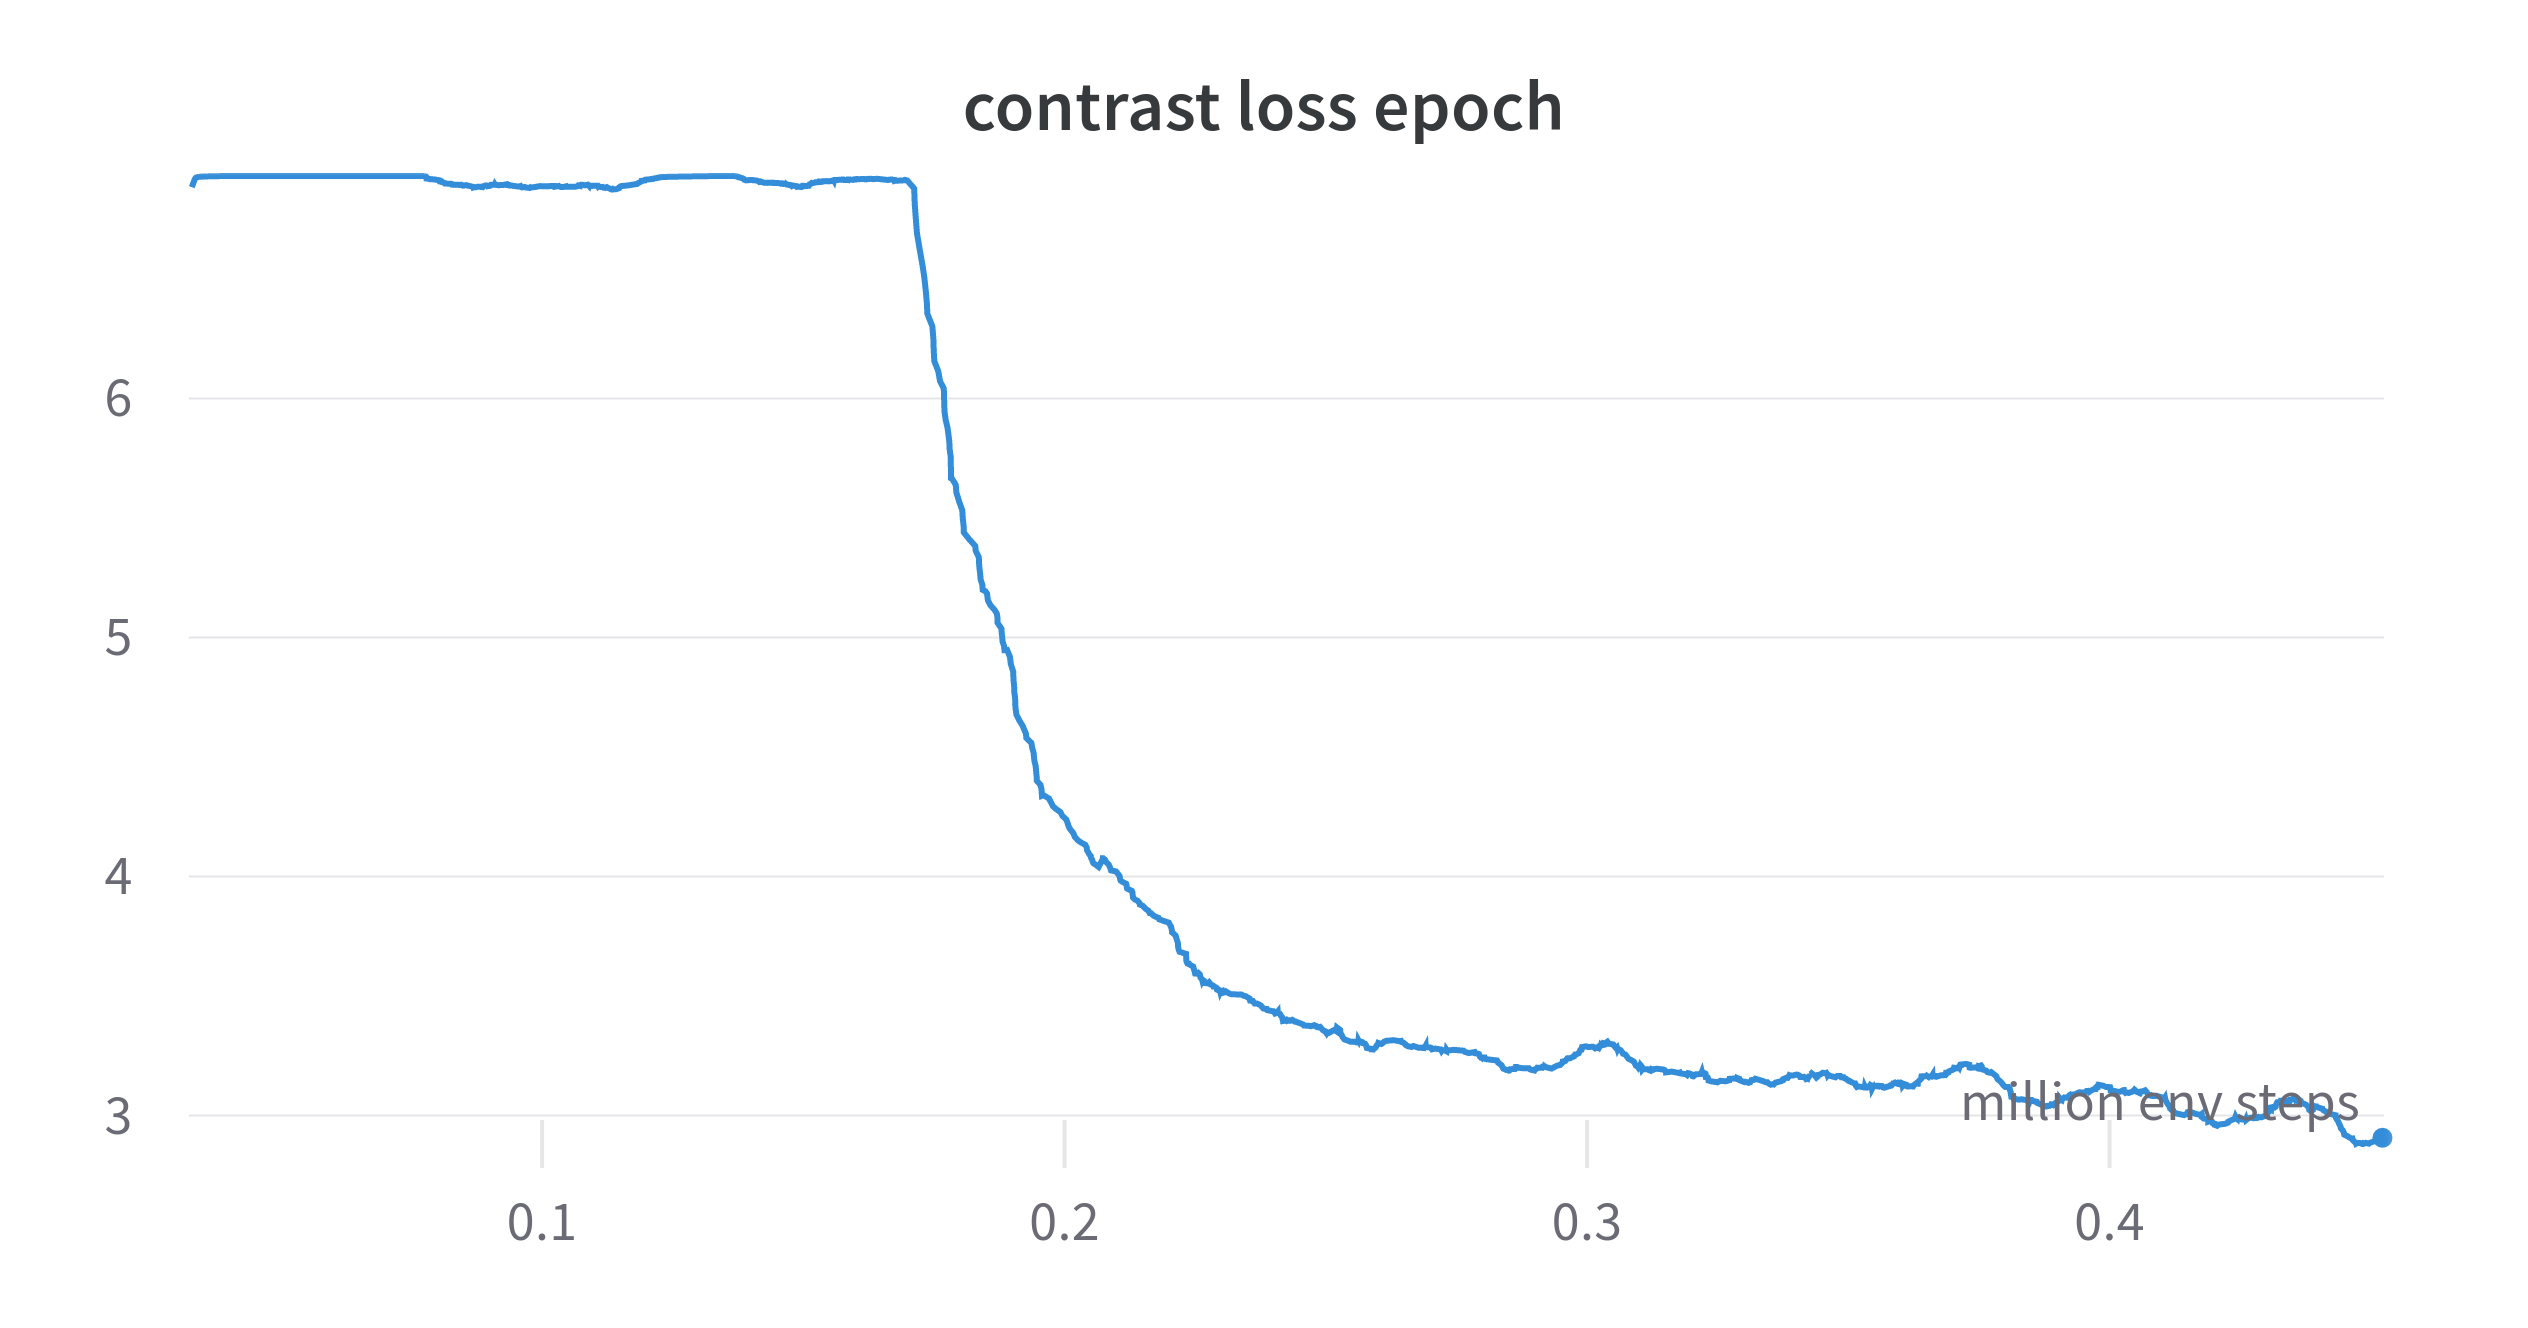
\includegraphics[width = 250pt]{contrast_loss_drop.png}
  \caption{Contrastive loss drops by a large amount in a short time}
\end{figure}

\begin{figure}[h]
  \centering
  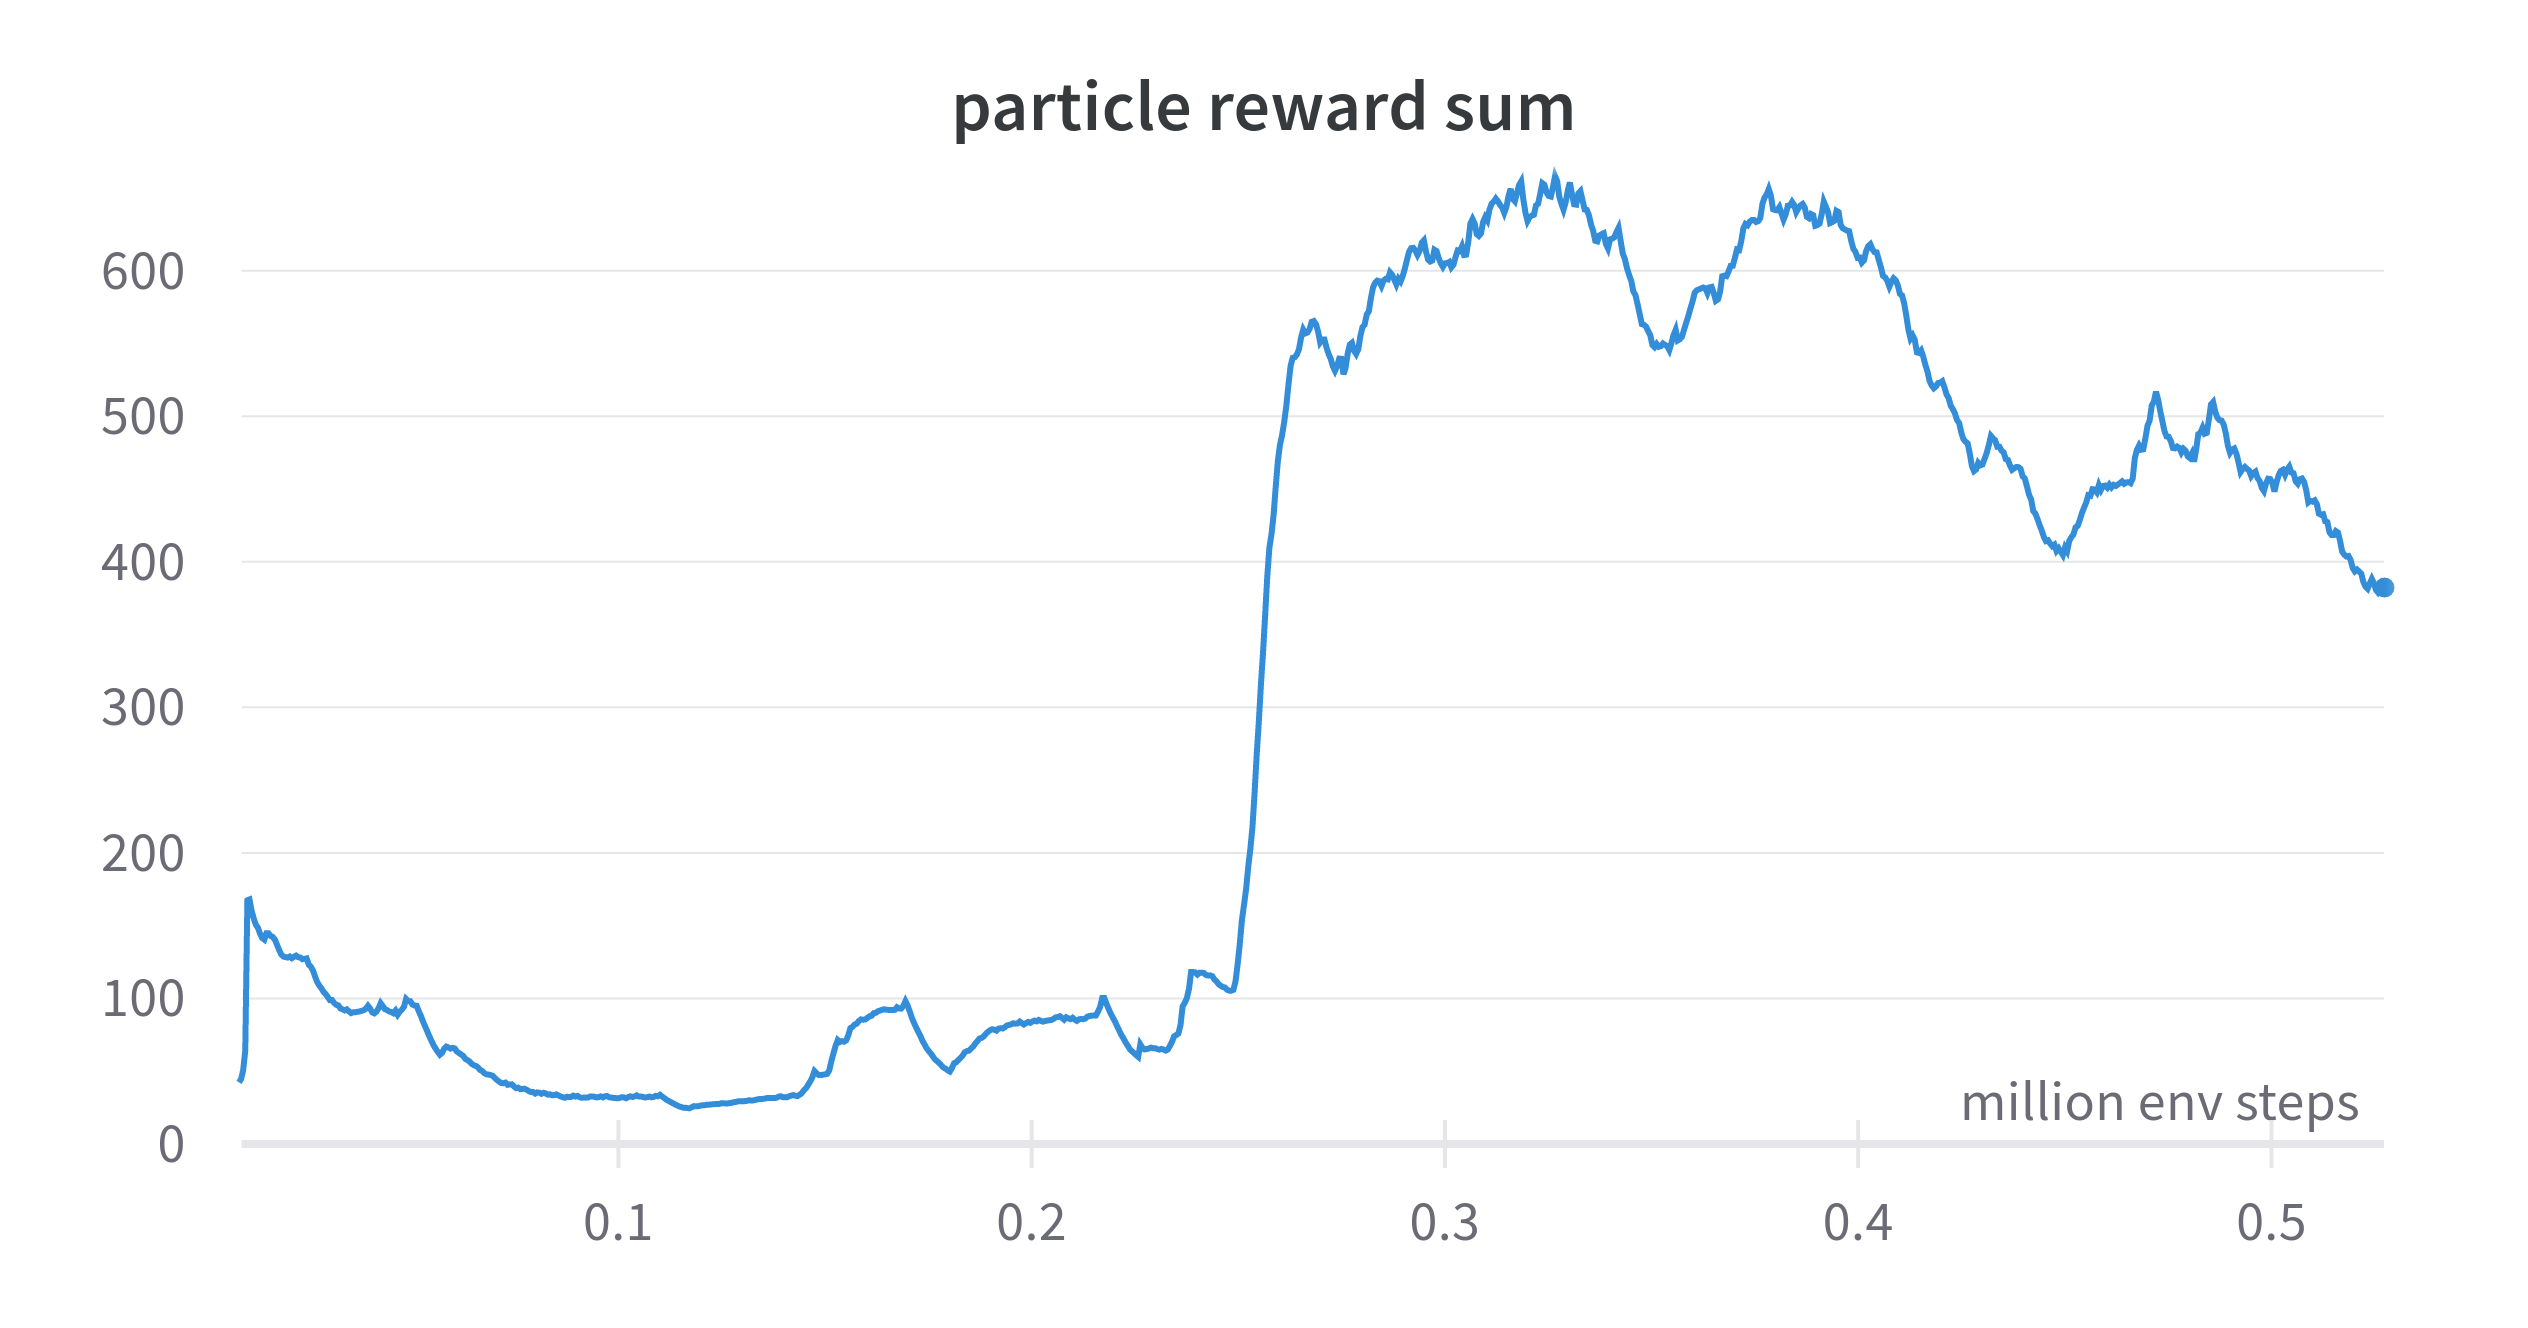
\includegraphics[width = 250pt]{particle_sum_contrast_loss_drop.png}
  \caption{Particle sum increases by a large margin once the encoder learns better representations}
\end{figure}

\noindent To avoid this otherwise inevitable collapse a variety of methods need to be applied and fine-tuned.\\
First the entropy term of the distribution of $\pi(\cdot|s)$, which is added to the PPO objective,
is never scaled down during training. This term rewards a small auxiliary loss 
for the entropy of the distribution.\\
The chosen scaling factor for this term is $0.01$ and should not be decayed without domain knowledge and careful
testing on when it is decay-able without risking policy collapse. Additionally the norm of the
gradient has to be clipped because it adds smoothness to the gradient~\cite{Zhang2020Why} and prevents
the policy from doing too big of an update step when the rewards increase rapidly.
For the maximum gradient norm
0.5 has worked best for the policy network and 10 for the encoder.\\
Choosing a low learning rate for the policy $\pi$ is also crucial to limit the update size.
During the pre-training phase the learning rate used to update $\pi$ is $1 * 10^{-4}$ and during the downstream task $3*10^{-4}$.\\
Auxiliary epochs also need to be modified in order to prevent policy collapse. If an auxiliary epoch happens
during the rapid increase of the rewards the policy can diverge a lot during the optimization of the value head $\pi_{aux}$.
Even though the behavior cloning loss term in $\mathcal{L}_{aux}$ helps the updates not diverge too far,
when reward scaling increases threefold it does not help enough. The KL divergence of the policy is measured
and if it exceeds a threshold $\delta = 0.01$ no further gradient updates are done during the auxiliary phase.\\
All of these techniques are required in order to stabilize PPG enough to work with APT and increase the unnormalized particle
reward over time.\\
Instead of pre-training for 250 million steps, this work trained for 62.5 million steps, skipping 4 frames~\cite{DBLP:journals/corr/abs-2102-03718} after each environment step.
This is partially necessary because of the Parallelism-Variance Dilemma which limits the number of parallel environments. 250
million training steps without frame skipping would have taken a month on a single NVIDIA-RTX6000 GPU,
which is the GPU used for the pre-training. Better or more GPUs do not
reduce the training time because the bottleneck is the interaction with the environment.
More CPUs do not scale because the parallelism hits its limit due to the required variance of
the state samples. This amount of computational time is sadly beyond the scope of this work, which takes a first 
look at the benefits and problems of unsupervised on-policy training has.

\begin{figure}[h]
  \centering
  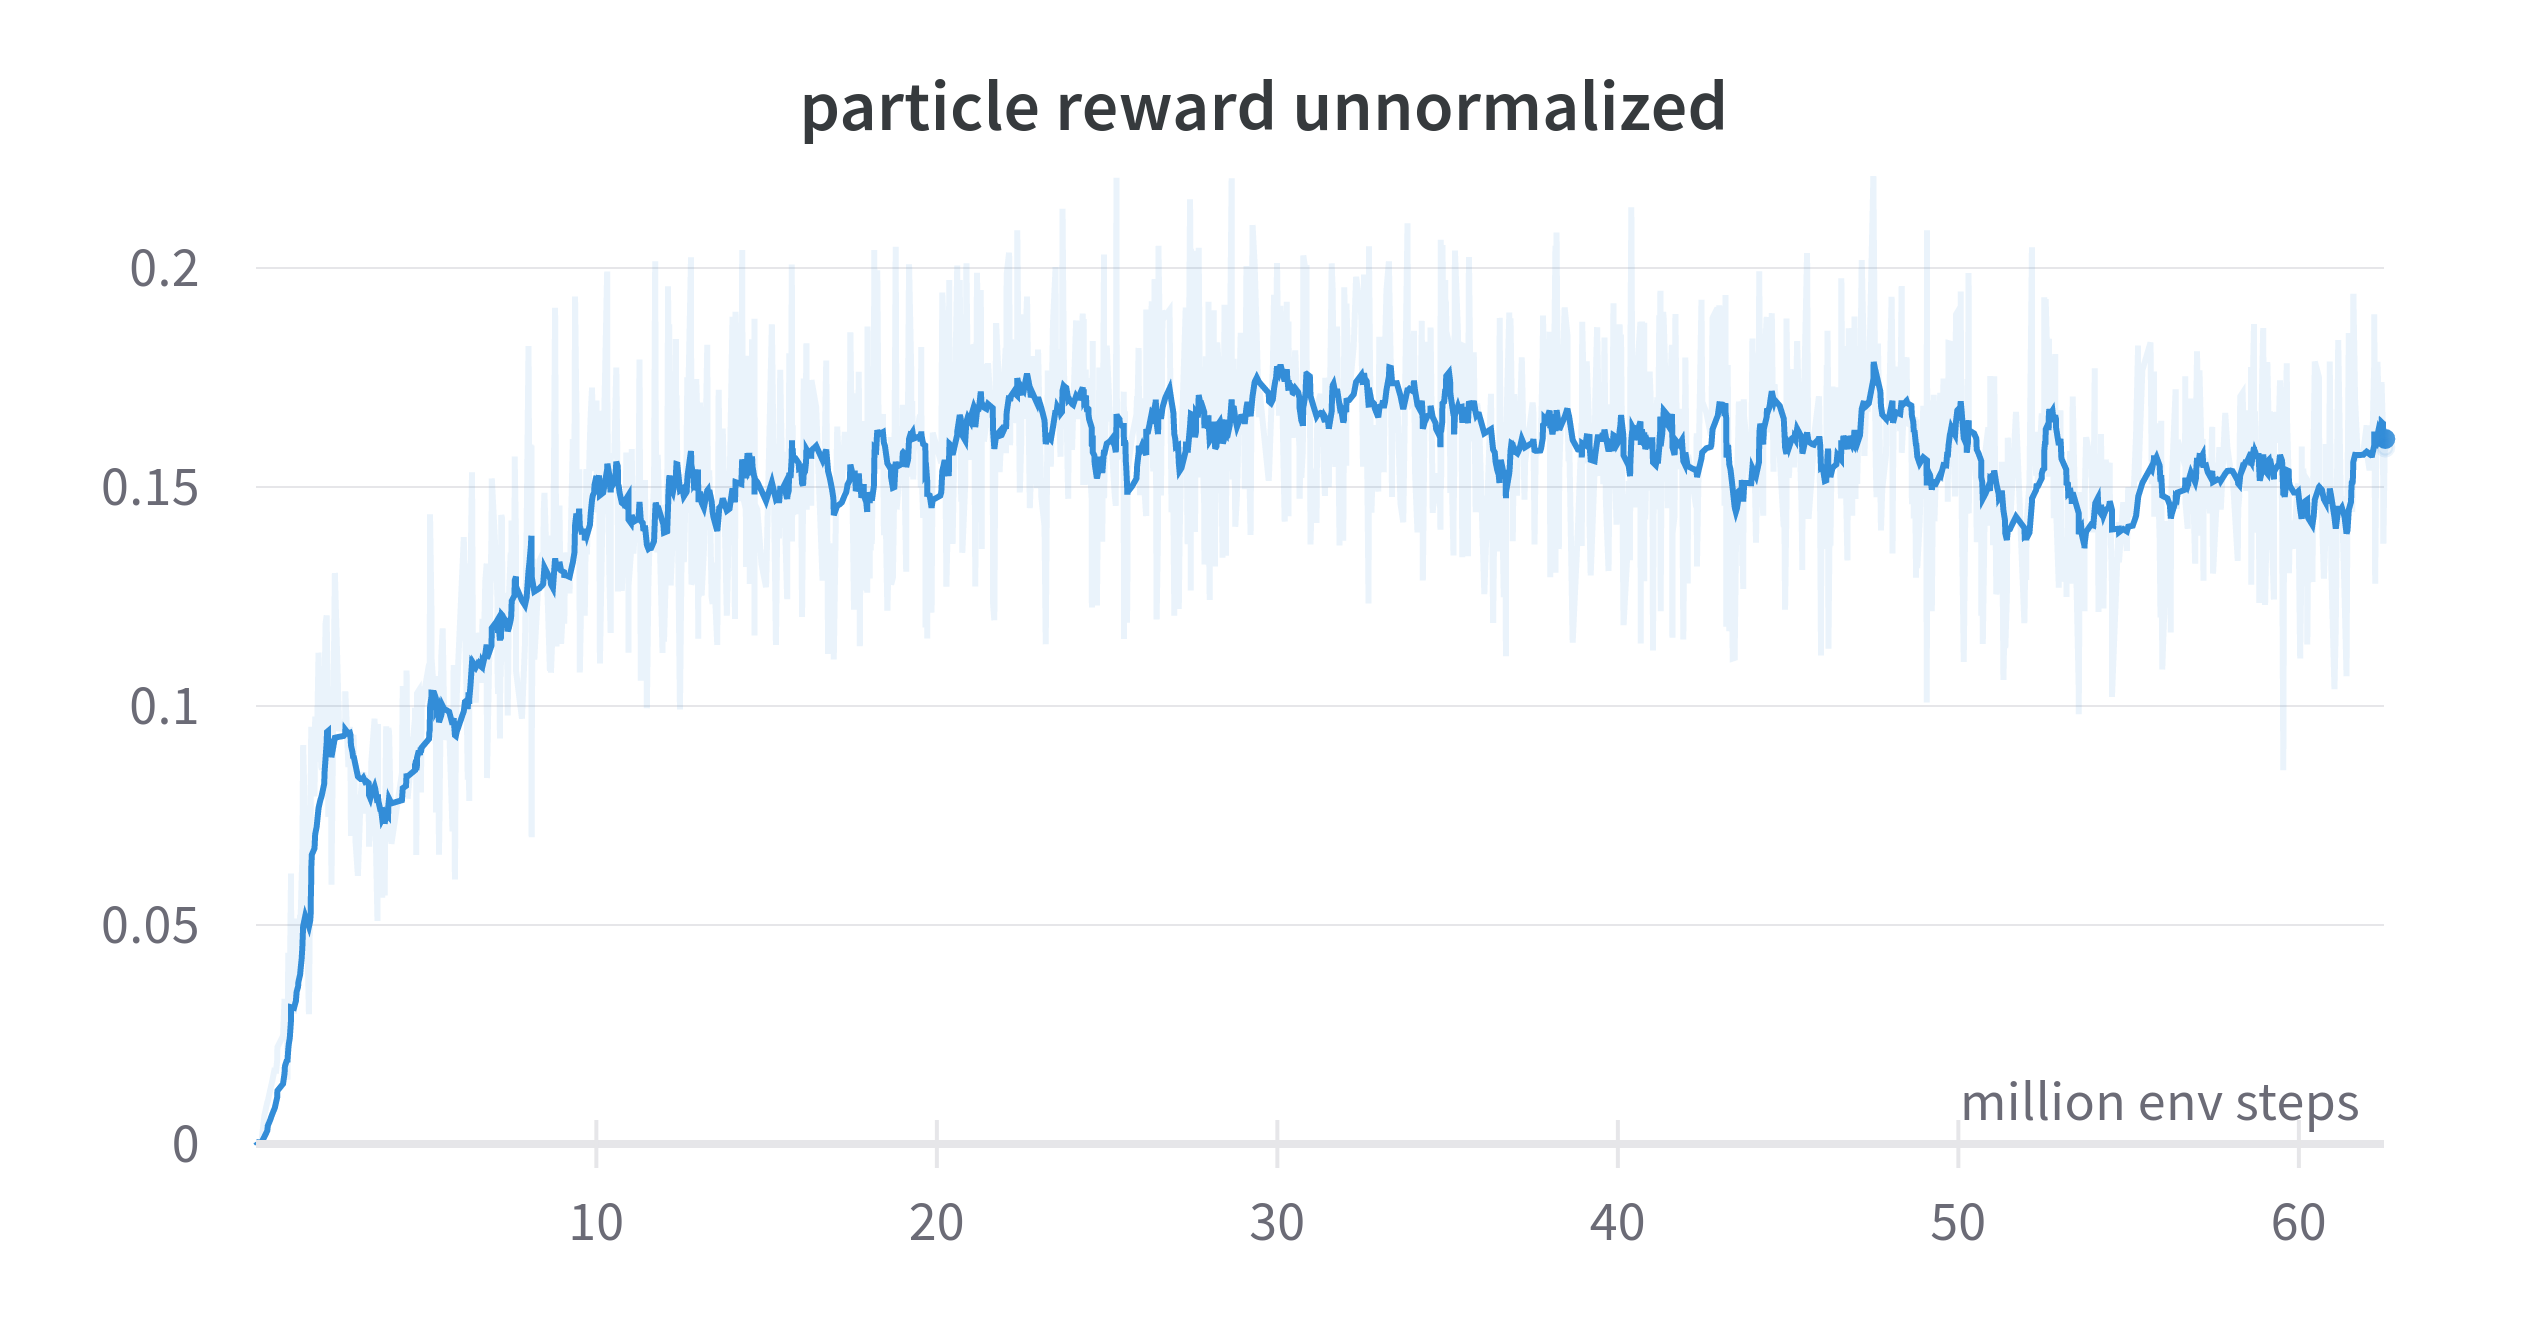
\includegraphics[width = 250pt]{part_rew.png}
  \caption{If the initial impending policy collapse is avoided by the techniques above, the particle reward rises and
  stays high for a long amount of time.}
\end{figure}

\begin{algorithm}[H]
\begin{algorithmic}[1]
\caption{APT with PPG Pseudocode}
\State Randomly Initialize encoder $f$
\State Randomly Initialize policy $\pi_\theta$ and state-value function $v_\psi$
\State Initialize empty representation buffer $D$
\State Initialize empty rollout buffer $B$
\State Initialize counter $i = 0$
\For{t = 1,2,..., T}
    \State Receive state $s_t$ from the environment
    \State Take action $a_t \sim \pi(\cdot|s_t)$, receive next state $s'_t$
    \State Ignore the reward $R_{t+1}$ from the environment
    \State $D \gets D \cup (s_t, a_t, s'_t)$
    \State $B \gets B \cup (s_t, a_t, s'_t, \pi_(a_t|s_t))$
    \State Sample minibatch from $D$ and train neural encoder $f$ on it
    \If{len(B) == rollout length}
        \For{batch $b\in B$}
            \State Compute particle-based entropy reward $R_{b}$
            \State $y_{b} \gets \hat A_\pi(s_{b}, a_{b})$
            \State Optimize $\mathcal{L}_{CLIP}$ w.r.t. the policys parameters $\theta$
            \State Optimize $\mathcal{L}_{value}$ w.r.t. the critics parameters $\psi$
        \EndFor
    \State Reinitialize empty rollout buffer $B$
    \State $i \gets i + 1$
    \EndIf
    \If{$i\mod N_\pi == 0$}
        \For{epoch = 1,2,...,$E_{aux}$}
            \State Optimize $\mathcal{L}_{aux}$ w.r.t. $\theta$ on all data in B
            \State Optimize $\mathcal{L}_{value}$ w.r.t. $\psi$ on all data in B
        \EndFor
    \EndIf
\EndFor
\end{algorithmic}
\end{algorithm}

\subsection{Evaluation}

\noindent After pre-training in such manner for 62.5 million steps we expose the policy $\pi$ to the downstream
reward function of the game Ms. Pac-Man and train the policy on it for 10 million environment steps.
The original APT paper reports a mean reward of $2827.1$ after 100 thousand training steps. On-policy algorithms
are not competitive in terms of sample efficiency, our approach only yields around $450$ after the same amount of
environmental steps. We therefore compare the success of the method by comparing
it to the 10 million steps benchmark of similar algorithms. Furthermore we compare
it to the same implementation without pre-training.\\
PPG ~\cite{DBLP:journals/corr/abs-2009-04416} does not provide benchmark results for Atari, but the original PPO
paper~\cite{DBLP:journals/corr/SchulmanWDRK17} was evaluated on it. Their results, on 10 million environment steps, or 40
million frames were a mean of $2096.5$ points in Ms. Pac-Man.
The results of this implementation of PPG had a mean of $1441.3$ without pre-training and $1212.9$ when pre-trained
before being exposed to the downstream task. This was averaged over 5 runs on a single seed.\\
Not only did the pre-training not actively increase performance, but it decreased the mean reward. 
Though the different runs had a lower variance than the ones which were not pre-trained, this is most
likely due to their common starting point, the policy after the pre-training phase.

\begin{figure}[h]
  \centering
  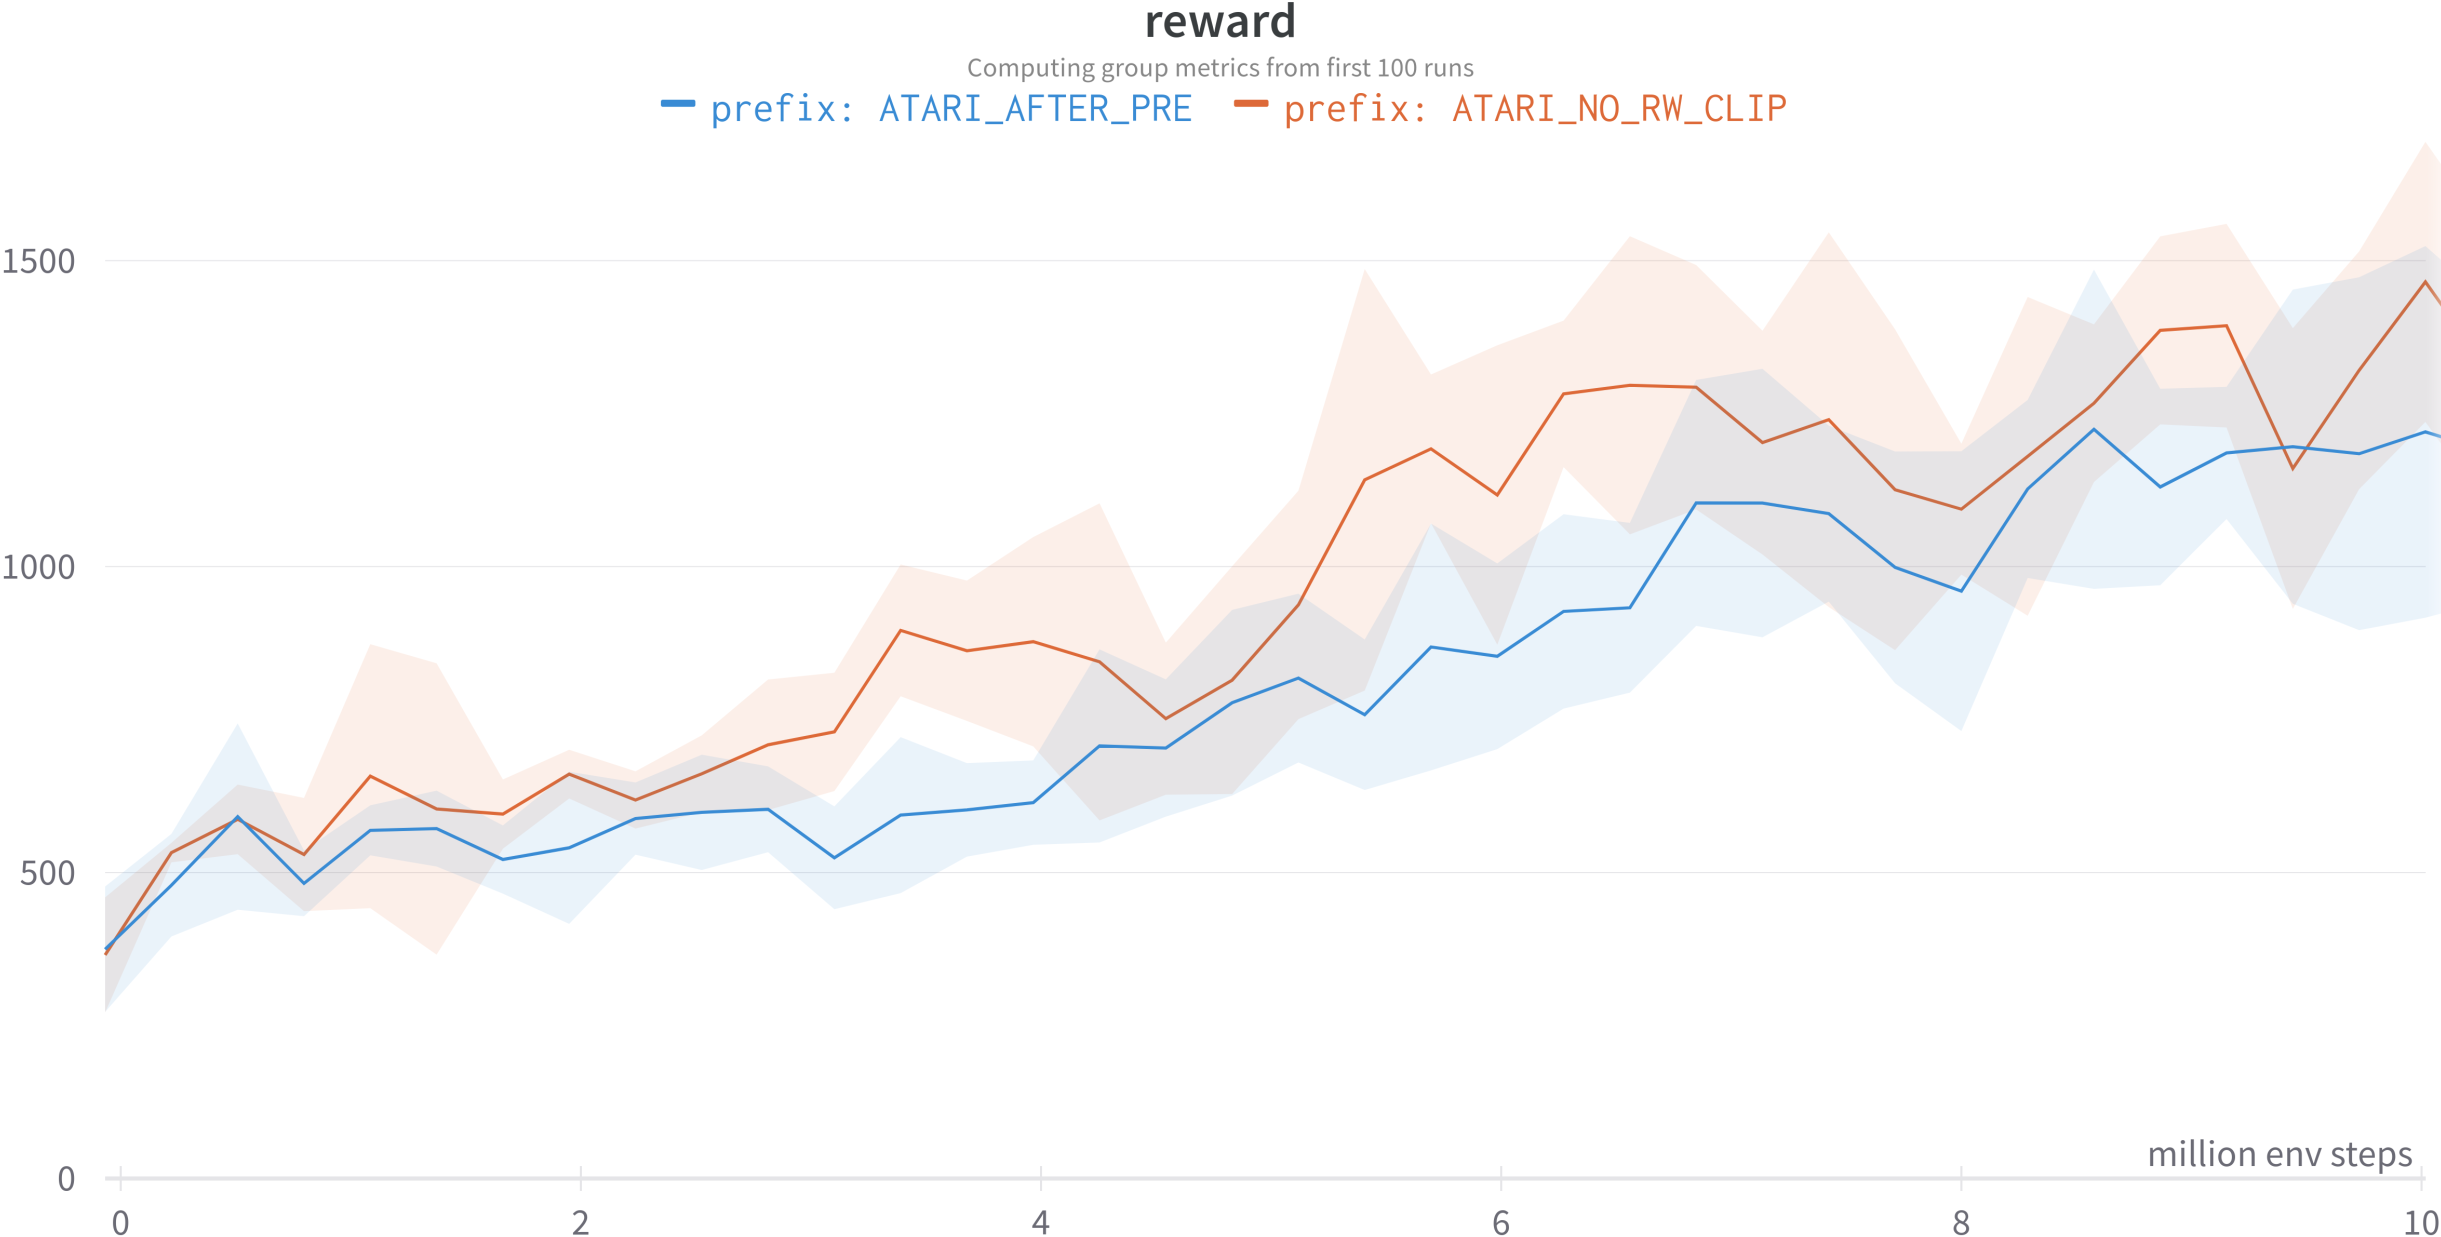
\includegraphics[width = 300pt]{result_fix.png}
  \caption{Results from pre-trained (blue) and without pre-training (orange). Standard deviation is also shown.}
\end{figure}


\noindent The authors mention in the APT paper that long pre-training is key to the success of the method, so using
frame skip might not accelerate learning meaningful representations enough to offset the shortened training time.\\
Performance actually went down after pre-training, which can have several of reasons. The most important one
is that we used frame skip instead of training for 250 million steps.
Furthermore the action-value function in APT is trained on the entire replay 
buffer on each step of the environment. This means there the difference in computation used is so large that it may just not
be compensable. To compensate this, on-policy algorithms are able to make use of higher learning rates, which is not
possible here due to the instability during pre-training. Especially when the contrastive loss goes down and
representations are pushed away further from each other, a higher learning rate leads to inevitable policy collapse and
is therefore not viable.
The difference in results compared to PPO is surprising considering that the network architecture is
from the original DQN-Paper~\cite{DBLP:journals/corr/MnihKSGAWR13} and only the value head was added. The hyperparameters used
have been taken from the PPG paper or from large scale studies~\cite{DBLP:journals/corr/abs-2006-05990} on the topic.
These hyperparameters might be optimized for the Procgen Benchmark~\cite{DBLP:journals/corr/abs-1912-01588} and therefore
might not work as well on Atari. The biggest difference is the clipping parameter $\epsilon$, which is set to $0.1$ for Atari in the
PPO paper. PPG recommends $0.2$ while the on-policy study~\cite{DBLP:journals/corr/abs-2006-05990} 
recommends starting with $0.25$.\\
In APT the authors suggest that reinitializing the network heads could improve performance if the magnitude of the rewards were shifted dramatically.
This was tested, but the results were worse than before.\\
Another possibility is that the results are very meaningful enough because the algorithm was evaluated on a single seed,
in a single game. Pre-training was also only done once due to runtime.
Most probably all the named factors had their influence on the results.

\section{Conclusion}

Instead of gaining benefits from combining of APT with PPG, the combined usage has turned out to be a worst of both worlds scenario.
The runtime can not be reduced drastically while preserving good results because of the Parallelism-Variance Dilemma. 
Also the instability of training eliminates most of the flexible choices related to the selection of hyperaparameters.\\
Off-policy algorithms outclass trust region on-policy methods when combined with APT by a large margin.
Due to their superior sample efficiency the off-policy algorithms have an advantage in all environments where
environments steps are expensive.\\
Reward calculated using off-policy APT are better estimates because the much
larger replay buffer can sample from more states. Therefore the states are compared
to a wider variety of other states, which makes its approximated particle-based entropy more accurate.
This and the shorter pre-training are likely scenarios on why the pre-trained agent performed worse.\\
PPG does not induce additional stability into the system, but rather the opposite. It is extremely prone to
policy collapse during the first few million environment steps of the pre-training phase. Due to
the contrastive loss function and the rewards computed from the representations, a vicious cycle of events
happens which the agent almost never recovers from.
Furthermore the Parallelism-Variance Dilemma limits the number of parallel environments that can used and therefore
the reduction in computation time.\\
The assumed benefits of the method proposed in this thesis are heavily outweighed by the disadvantages it provides.
Combating these drawbacks cut into the flexibility of the approach and thereby eliminate almost all advantages
on-policy algorithms have.
The original off-policy algorithm in APT outclasses the method proposed in this thesis. It better
in terms of sample efficiency, is more scaleable and is less vulnerable to the Variance-Parallelism Dilemma.

\newpage
\bibliography{refs}{}
\bibliographystyle{plain}
\newpage
\section{Appendix}
All code is appended here, but is also accessible at this Github: \url{https://github.com/tnfru/unsupervised-on-policy/}\\
It can be installed via pip too, link to Pypi package: \url{https://pypi.org/project/unsupervised-on-policy/}
\begin{figure}[h]
  \centering
  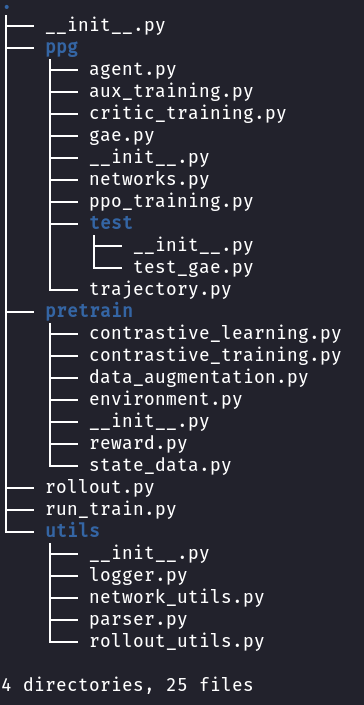
\includegraphics[width = 150pt]{code_struct.png}
  \caption{Code Structure}
\end{figure}
\newpage

run\_train.py
\begin{lstlisting}[language=Python]
from ppg.agent import Agent
from unsupervised_on_policy.rollout import run_timesteps
import pretrain.environment as environment
from utils.parser import parse_args
import sys


def main():
    args = sys.argv[1:]
    args = parse_args(args)

    config = {'policy_clip': 0.25,
              'kl_max': None,
              'kl_max_aux': None,
              'clip_reward': True,
              'beta': 1,
              'val_coeff': 1e-2,
              'train_iterations': 1,
              'entropy_coeff': 0.01,
              'entropy_min': 0.01,
              'entropy_decay': 0.9999,
              'grad_norm': 10,
              'grad_norm_ppg': 0.5,
              'critic_lr': 1e-3,
              'actor_lr': 3e-4,
              'aux_freq': 32,
              'aux_iterations': 3,
              'gae_lambda': 0.95,
              'batch_size': 32,
              'target_batch_size': 32,
              'use_wandb': True,
              'discount_factor': 0.99,
              'height': 84,
              'width': 84,
              'action_dim': 18,
              'contrast_lr': 1e-3,
              'temperature': 0.1,
              'frames_to_skip': 4,
              'stacked_frames': 4,
              'steps_before_repr_learning': 1600,
              'replay_buffer_size': 10000,
              'is_pretrain': False if args.skip_pretrain else True,
              'num_envs': 16,
              'prefix': args.prefix,
              'path': args.model_path
              }

    if config['is_pretrain']:
        config.update({
            'batch_size': 512,
            'target_batch_size': 512,
            'entropy_min': 0.01,
            'actor_lr': 1e-4,
            'kl_max_aux': 0.01,  # stability in pretrain
        })

    config.update({
        'rollout_length': max(config['target_batch_size'], 256)
    })

    SEED = 1337
    NUM_TIMESTEPS = 250_000_000

    environment.seed_everything(SEED)
    env = environment.create_env(config)
    agent = Agent(env, config=config, load=args.load)

    run_timesteps(agent, NUM_TIMESTEPS, pretrain=config['is_pretrain'])


if __name__ == '__main__':
    main()
\end{lstlisting}

\newpage
rollout.py
\begin{lstlisting}[language=Python]
import torch as T
import numpy as np
from einops import rearrange

from pretrain.reward import calc_pretrain_rewards
from utils.logger import log_episode
from pretrain.contrastive_training import train_contrastive_batch
from utils.rollout_utils import append_task_reward
from utils.rollout_utils import fetch_terminal_state
from utils.rollout_utils import get_idx
from utils.rollout_utils import is_repr_learn_phase
from utils.rollout_utils import is_training_step


def run_timesteps(agent: T.nn.Module, num_timesteps: int, pretrain: bool):
    """
    Runs one episode in the set environment
    Args:
        agent: agent handling the episode
        num_timesteps: steps to train for
        pretrain: if reward is given by environment or calculated in a self
        supervised fashion
    Returns: new number of steps done
    """
    total_steps_done = 0
    num_envs = agent.config['num_envs']
    rewards = np.zeros(num_envs).astype(float)
    eps_lengths = np.zeros(num_envs).astype(int)

    state = T.from_numpy(agent.env.reset()).to(agent.device).float()
    state = rearrange(state, 'envs h w c -> envs c h w')

    while total_steps_done < num_timesteps:
        action, log_prob, aux_val, log_dist = agent.get_action(state)
        next_state, reward, done, info = agent.env.step(action)
        next_state = T.from_numpy(next_state).to(agent.device).float()
        next_state = rearrange(next_state, 'envs h w c -> envs c h w')

        rewards = rewards + reward
        state = state.cpu()
        agent.append_to_replay_buffer(state, total_steps_done)

        if is_repr_learn_phase(agent.config, total_steps_done):
            train_contrastive_batch(agent, total_steps_done)

        if is_training_step(agent.config, total_steps_done):
            with T.no_grad():
                states = agent.trajectory.states.to(agent.device)

                agent.trajectory.state_vals = agent.critic(
                    states).squeeze().detach().cpu()

            if pretrain:
                calc_pretrain_rewards(agent)

            agent.learn(total_steps_done)

        idx = get_idx(agent, total_steps_done)
        if done.any():
            log_episode(agent, rewards, eps_lengths, total_steps_done, done,
                        info)
            terminal_state = fetch_terminal_state(next_state, num_envs, done,
                                                  info)

            agent.trajectory.append_step(state, action, terminal_state, done,
                                         log_prob, aux_val, log_dist, idx)
        else:
            agent.trajectory.append_step(state, action, next_state.cpu(), done,
                                         log_prob, aux_val, log_dist, idx)
        append_task_reward(agent, reward, idx)
        state = next_state
        total_steps_done += 1
        eps_lengths = eps_lengths + 1

    return total_steps_done
\end{lstlisting}


\newpage
agent.py
\begin{lstlisting}[language=Python]

import torch as T
from torch.distributions.categorical import Categorical
import os
import wandb
import gym

from ppg.networks import CriticNet, PPG_DQN_ARCH
from ppg.trajectory import Trajectory
from ppg.aux_training import train_aux_epoch
from ppg.ppo_training import train_ppo_epoch
from ppg.critic_training import train_critic_epoch
from pretrain.reward import ParticleReward
from pretrain.data_augmentation import DataAugment
from pretrain.contrastive_learning import ContrastiveLearner, ContrastiveLoss
from utils.network_utils import get_loader
from utils.logger import init_logging, log_entropy_coeff, log_ppo_env_steps, \
    log_steps_done
from utils.rollout_utils import get_idx

try:
    from apex.optimizers import FusedAdam as Adam

    print('Using APEX optimizer')
except ModuleNotFoundError:
    from torch.optim import Adam

    print('Apex Optimizers not installed, defaulting to PyTorch Optimizer')


class Agent(T.nn.Module):
    def __init__(self, env: gym.envs, config: dict, load=False,
                 load_new_config=False):
        """
        Agent class for PPG + APT
        Args:
            env: gym environment to interact with
            config: configuration data
            load: load from previous run
            load_new_config: load a new config file
        """
        super().__init__()
        self.env = env
        self.metrics = {}

        self.actor = PPG_DQN_ARCH(config['action_dim'],
                                  config['stacked_frames'])
        self.actor_opt = Adam(self.actor.parameters(),
                              lr=config['actor_lr'])
        self.critic = CriticNet(config)
        self.critic_opt = Adam(self.critic.parameters(),
                               lr=config['critic_lr'])
        self.contrast_net = ContrastiveLearner(config)
        self.contrast_opt = Adam(self.contrast_net.parameters(),
                                 lr=config['contrast_lr'])
        self.contrast_loss = ContrastiveLoss(config)
        self.data_aug = DataAugment(config)
        self.reward_function = ParticleReward()
        self.trajectory = Trajectory(config)

        self.config = config
        self.entropy_coeff = config['entropy_coeff']
        self.use_wandb = config['use_wandb']
        self.AUX_WARN_THRESHOLD = 100
        self.steps = 0
        self.path = config['path']

        if config['is_pretrain']:
            self.replay_buffer = T.zeros(config['replay_buffer_size'], config[
                'stacked_frames'], config['height'], config['width'])

        self.device = T.device(
            'cuda' if T.cuda.is_available() else 'cpu')
        self.to(self.device)

        init_logging(config, self, config['prefix'])

        if load:
            self.load_model()

            if load_new_config:
                entropy_coeff = self.entropy_coeff
                self.config = config
                self.entropy_coeff = entropy_coeff

    @T.no_grad()
    def get_action(self, state):
        """
        Args:
            state: torch tensor, current observation from environment
        Returns:
            action: int, selected action
            log_prob: float, log probability of the selected action
            aux value: float, state value as predicted by ppg value head 
            log_dist: torch tensor, log distribution over actions
        """
        action_probs, aux_value = self.actor(state)
        aux_value = aux_value.squeeze().cpu()

        action_dist = Categorical(logits=action_probs)
        action = action_dist.sample()
        log_prob = action_dist.log_prob(action).squeeze().cpu()
        action = action.squeeze().cpu()
        log_dist = action_dist.probs.log().squeeze().cpu()

        return action, log_prob, aux_value, log_dist

    def learn(self, total_steps_done):
        """
        Trains the different networks on the collected trajectories
        """
        with T.no_grad():
            num_envs = self.config['num_envs']
            final_states = self.trajectory.next_states[-num_envs:].to(
                self.device)
            last_state_vals = self.critic(final_states).squeeze().cpu()

        self.trajectory.calc_advantages(self.config, last_state_vals)

        self.ppo_training_phase()
        self.steps += self.config['train_iterations']

        if self.steps >= self.config['aux_freq']:
            self.aux_training_phase()
            self.steps = 0

        self.entropy_coeff = max(self.entropy_coeff * self.config[
            'entropy_decay'], self.config['entropy_min'])
        self.log_training(total_steps_done)

        self.forget()
        self.save_model()

    def ppo_training_phase(self):
        """ Trains the actor network on the PPO Objective """
        loader = get_loader(dset=self.trajectory, config=self.config)

        for epoch in range(self.config['train_iterations']):
            train_ppo_epoch(agent=self, loader=loader)
            train_critic_epoch(agent=self, loader=loader)

    def aux_training_phase(self):
        """ Trains the actor network on the PPG auxiliary Objective """
        self.trajectory.is_aux_epoch = True

        loader = get_loader(dset=self.trajectory, config=self.config)

        for aux_epoch in range(self.config['aux_iterations']):
            train_aux_epoch(agent=self, loader=loader)
            train_critic_epoch(agent=self, loader=loader, is_aux=True)

        self.trajectory.is_aux_epoch = False

    def forget(self):
        """ Removes the collected data after training"""
        self.trajectory = Trajectory(self.config)

    def append_to_replay_buffer(self, state, steps_done):
        if self.config['is_pretrain']:
            idx = get_idx(self, steps_done, replay_buffer=True)
            self.replay_buffer[idx] = state

    def save_model(self):
        os.makedirs(self.path, exist_ok=True)
        PATH = self.path + '/agent_latest.pt'
        T.save(self.state_dict(), PATH)

    def load_model(self):
        print('Loading Model...')
        PATH = self.path + '/agent_latest.pt'
        self.load_state_dict(T.load(PATH))
        print('Model loaded. Starting training.')

    def log_training(self, total_steps_done):
        log_ppo_env_steps(self, total_steps_done)
        log_steps_done(self, total_steps_done)
        log_entropy_coeff(self)
        self.log_metrics()

    def log_metrics(self):
        if self.use_wandb:
            wandb.log(self.metrics)
            self.metrics = {}
\end{lstlisting}

\newpage
aux\_training.py
\begin{lstlisting}[language=Python]
import torch as T
import torch.nn.functional as F
from torch.distributions.categorical import Categorical

from utils.network_utils import data_to_device, approx_kl_div
from utils.network_utils import do_accumulated_gradient_step
from utils.logger import warn_about_aux_loss_scaling, log_aux, log_nan_aux


def train_aux_epoch(agent: T.nn.Module, loader: T.utils.data.DataLoader):
    """
    Trains actor on PPG auxiliary objective for one epoch
    Args:
        agent: agent to be trained
        loader: includes the data to be trained on
    """
    num_batches = len(loader)

    for batch_idx, rollout_data in enumerate(loader):
        states, _, aux_returns, log_dists = data_to_device(rollout_data,
                                                           agent.device)
        aux_returns = aux_returns.unsqueeze(1)

        train_aux_batch(agent=agent, states=states,
                        expected_returns=aux_returns, old_log_probs=log_dists,
                        batch_idx=batch_idx, num_batches=num_batches)


def train_aux_batch(agent: T.nn.Module, states: T.tensor,
                    expected_returns: T.tensor,
                    old_log_probs: T.tensor,
                    batch_idx, num_batches):
    """
    Trains actor on PPG auxiliary objective for one batch
    Args:
        states: representation of the environment
        expected_returns: aux state values + aux advantages
        old_log_probs: log probs at the time of action selection
    """
    config = agent.config
    action_logits, aux_values = agent.actor(states)

    if T.isnan(action_logits).any():
        log_nan_aux(agent)
        return

    action_dist = Categorical(logits=action_logits)
    log_probs = action_dist.probs.log()
    kl_div = approx_kl_div(log_probs, old_log_probs, is_aux=True)

    aux_value_loss = F.mse_loss(aux_values, expected_returns)
    aux_value_loss = aux_value_loss * config['val_coeff']

    if aux_value_loss > agent.AUX_WARN_THRESHOLD:
        warn_about_aux_loss_scaling(aux_value_loss)

    aux_loss = aux_value_loss + kl_div * config['beta']

    if config['kl_max_aux'] is None or kl_div < config['kl_max_aux']:
        # If KL divergence is too big we don't take gradient steps
        do_accumulated_gradient_step(agent.actor, agent.actor_opt, aux_loss,
                                     config, batch_idx, num_batches)

    if agent.use_wandb:
        log_aux(agent, aux_values, aux_loss, kl_div, config['kl_max'])
\end{lstlisting}

\newpage
critic\_train.py
\begin{lstlisting}[language=Python]
import torch as T
import torch.nn.functional as F
from utils.logger import log_critic

from utils.network_utils import do_accumulated_gradient_step
from utils.network_utils import data_to_device


def train_critic_epoch(agent: T.nn.Module, loader: T.utils.data.DataLoader,
                       is_aux=False):
    """
    Trains the critic for one epoch on the score function (MSE usually)
    Args:
        agent: agent to train
        loader: contains the data to train on
        is_aux: if it is an auxiliary epoch or not
    """
    num_batches = len(loader)
    for batch_idx, rollout_data in enumerate(loader):
        if is_aux:
            states, expected_returns, _, _ = data_to_device(
                rollout_data, agent.device)
        else:
            states, actions, expected_returns, _, _ = data_to_device(
                rollout_data, agent.device)
        expected_returns = expected_returns.unsqueeze(1)
        train_critic_batch(agent=agent, states=states,
                           expected_returns=expected_returns,
                           batch_idx=batch_idx, num_batches=num_batches)


def train_critic_batch(agent, states: T.tensor, expected_returns: T.tensor,
                       batch_idx, num_batches):
    """
    Trains the critic for one batch on the score function (MSE usually)
    Args:
        states: representations of the environment
        expected_returns: state values + advantages
    """
    config = agent.config
    state_values = agent.critic(states)

    critic_loss = F.mse_loss(state_values, expected_returns)

    do_accumulated_gradient_step(agent.critic, agent.critic_opt, critic_loss,
                                 config, batch_idx, num_batches)

    log_critic(agent, critic_loss, state_values)
\end{lstlisting}
\newpage



gae.py
\begin{lstlisting}[language=Python]
import torch as T
from einops import rearrange


def calculate_advantages(rewards: T.tensor, state_vals: T.tensor,
                         dones: T.tensor, last_state_val: T.tensor,
                         config: dict):
    """
    Calculated Advantages via Generalized Advantage Estimation (GAE)
    https://arxiv.org/abs/1506.02438
    Args:
        rewards: reward obtained
        state_vals: predicted state values
        last_state_val: value of the next state of the last step
        dones: if terminal state or not
        config: configuration file
    Returns: advantages over the given timesteps
    """
    discount_factor = config['discount_factor']
    gae_lambda = config['gae_lambda']

    advantages = []
    advantage = 0
    next_state_value = last_state_val
    num_envs = config['num_envs']

    rewards = rearrange(rewards, '(step env) -> step env ', env=num_envs)
    state_vals = rearrange(state_vals, '(step env) -> step env ', env=num_envs)
    dones = rearrange(dones, '(step env) -> step env ', env=num_envs)

    for reward, state_val, done in zip(reversed(rewards), reversed(state_vals),
                                       reversed(dones)):
        td_error = reward + (
                1 - done) * discount_factor * next_state_value - state_val
        advantage = td_error + discount_factor * gae_lambda * advantage
        advantages.insert(0, advantage)
        next_state_value = state_val

    advantages = T.stack(advantages)
    advantages = rearrange(advantages, 'step env -> (step env) ', env=num_envs)

    return advantages
\end{lstlisting}
\newpage

networks.py
\begin{lstlisting}[language=Python]
import torch as T
import torch.nn as nn
from einops import reduce
from einops.layers.torch import Rearrange


class CriticNet(nn.Module):
    def __init__(self, config):
        super().__init__()
        self.conv1 = nn.Sequential(
            nn.Conv2d(config['stacked_frames'], 64, 3, bias=False),
            nn.BatchNorm2d(64),
            nn.ReLU(inplace=True)
        )

        self.conv2 = nn.Sequential(
            nn.Conv2d(64, 64, 3, bias=False),
            nn.BatchNorm2d(64),
            nn.ReLU(inplace=True)
        )

        self.conv3 = nn.Sequential(
            nn.Conv2d(64, 128, 3, bias=False),
            nn.BatchNorm2d(128),
            nn.ReLU(inplace=True)
        )

        self.backbone = nn.Sequential(
            self.conv1,
            self.conv2,
            self.conv3
        )

        self.head = nn.Sequential(
            nn.Linear(128, 1)
        )

        self.device = T.device(
            'cuda' if T.cuda.is_available() else 'cpu')
        self.to(self.device)

    def forward(self, x):
        x = x / 255 - 0.5
        x = self.backbone(x)
        x = global_avg_pool(x)
        x = self.head(x)

        return x


class PPG_DQN_ARCH(nn.Module):
    def __init__(self, action_dim, state_dim):
        """
        Phasic Policy Gradient Network
        Args:
            action_dim: number of available actions
            state_dim: number of channels of state / observation
        """
        super().__init__()
        self.conv1 = nn.Sequential(
            nn.Conv2d(state_dim, 16, 8, stride=4),
            nn.ReLU(inplace=True)
        )

        self.conv2 = nn.Sequential(
            nn.Conv2d(16, 32, 4, stride=2),
            nn.ReLU(inplace=True)
        )

        self.mlp = nn.Sequential(
            Rearrange('b c h w -> b (c h w)'),
            nn.Linear(2592, 256),
            nn.ReLU(inplace=True)
        )

        self.backbone = nn.Sequential(
            self.conv1,
            self.conv2,
            self.mlp
        )

        self.action_head = nn.Sequential(
            nn.Linear(256, action_dim)
        )

        self.val_head = nn.Sequential(
            nn.Linear(256, 1)
        )

        with T.no_grad():
            # see https://arxiv.org/abs/2006.05990 network architecture
            self.action_head[0].weight /= 100
            self.val_head[0].weight /= 100

        self.device = T.device(
            'cuda' if T.cuda.is_available() else 'cpu')
        self.to(self.device)

    def forward(self, x):
        x = x / 255 - 0.5
        x = self.backbone(x)
        action_values = self.action_head(x)
        state_values = self.val_head(x)

        return action_values, state_values


class PPG(nn.Module):
    def __init__(self, action_dim, state_dim):
        """
        Phasic Policy Gradient Network
        Args:
            action_dim: number of available actions
            state_dim: number of channels of state / observation
        """
        super().__init__()
        self.conv1 = nn.Sequential(
            nn.Conv2d(state_dim, 64, 3, bias=False),
            nn.BatchNorm2d(64),
            nn.ReLU(inplace=True)
        )

        self.conv2 = nn.Sequential(
            nn.Conv2d(64, 64, 3, bias=False),
            nn.BatchNorm2d(64),
            nn.ReLU(inplace=True)
        )

        self.conv3 = nn.Sequential(
            nn.Conv2d(64, 128, 3, bias=False),
            nn.BatchNorm2d(128),
            nn.ReLU(inplace=True)
        )

        self.backbone = nn.Sequential(
            self.conv1,
            self.conv2,
            self.conv3
        )

        self.action_head = nn.Sequential(
            nn.Linear(128, action_dim)
        )

        self.val_head = nn.Sequential(
            nn.Linear(128, 1)
        )

        self.device = T.device(
            'cuda' if T.cuda.is_available() else 'cpu')
        self.to(self.device)

    def forward(self, x):
        x = self.backbone(x)
        x = global_avg_pool(x)
        action_values = self.action_head(x)
        state_values = self.val_head(x)

        return action_values, state_values


def global_avg_pool(values):
    """
    Performs the global average pooling operation
    Args:
        values: values to average
    Returns: chanel wise mean
    """
    return reduce(values, 'bs c h w -> bs c', 'mean')
\end{lstlisting}
\newpage


ppo\_training.py
\begin{lstlisting}
import torch as T
from torch.distributions.categorical import Categorical

from utils.network_utils import data_to_device, approx_kl_div
from utils.network_utils import do_accumulated_gradient_step
from utils.logger import log_ppo


def train_ppo_epoch(agent: T.nn.Module, loader: T.utils.data.DataLoader):
    """
    Trains actor on PPO surrogate objective for one epoch
    Args:
        agent: agent to be trained
        loader: includes the data to be trained on
    """
    num_batches = len(loader)

    for batch_idx, rollout_data in enumerate(loader):
        states, actions, expected_returns, advantages, log_probs = data_to_device(
            rollout_data, agent.device)

        train_ppo_batch(agent, states, actions, log_probs, advantages,
                        batch_idx, num_batches)


def train_ppo_batch(agent, states: T.tensor, actions: T.tensor,
                    old_log_probs: T.tensor, advantages: T.tensor,
                    batch_idx, num_batches):
    """
    Trains actor on PPO surrogate objective for one batch
    Args:
        states: representation of the environment
        actions: selected action for the respective states
        advantages: advantages of the selected action in their states
        old_log_probs: log probs at the time of action selection
            old_aux_value: aux state value
    """
    config = agent.config
    action_probs, _ = agent.actor(states)
    action_dist = Categorical(logits=action_probs)
    log_probs = action_dist.log_prob(actions)

    # entropy for exploration
    entropy_loss = entropy_objective(action_dist, agent.entropy_coeff)

    # log trick for efficient computational graph during backprop
    ratio = T.exp(log_probs - old_log_probs)
    ppo_loss = ppo_objective(advantages, ratio, config['policy_clip'])

    objective = ppo_loss + entropy_loss

    kl_div = approx_kl_div(log_probs, old_log_probs, is_aux=False)

    if config['kl_max'] is None or kl_div < config['kl_max']:
        # If KL divergence is too big we don't take gradient steps
        do_accumulated_gradient_step(agent.actor, agent.actor_opt, objective,
                                     config, batch_idx, num_batches,
                                     retain_graph=True)

    if agent.use_wandb:
        log_ppo(agent, entropy_loss, kl_div, config['kl_max'])


# Both objectives flip the sign to turn their objective into a loss
# This is because we want to do gradient ascent on the objectives, but
# optimizers in PyTorch generally do gradient descent

def ppo_objective(advantages, ratio, policy_clip):
    """
    Calculates the PPO CLIP objective as loss
    Args:
        advantages: advantages of the selected actions
        ratio: importance sampling ratio between new and old policy
        policy_clip: maximum allowed change from old policy
    """
    weighted_objective = ratio * advantages
    clipped_objective = ratio.clamp(1 - policy_clip,
                                    1 + policy_clip) * advantages
    ppo_loss = -T.min(weighted_objective, clipped_objective).mean()

    return ppo_loss


def entropy_objective(
        action_distribution: T.distributions.categorical.Categorical,
        entropy_coeff: float):
    """
    Entropy for exploration on PPO objective
    Args:
        action_distribution: distribution over the actions
        entropy_coeff: scaling factor
    Returns:
    """
    entropy_loss = -action_distribution.entropy().mean() * entropy_coeff

    return entropy_loss
\end{lstlisting}
\newpage


trajectory.py
\begin{lstlisting}
import torch as T

from ppg.gae import calculate_advantages
from utils.network_utils import normalize


class Trajectory(T.utils.data.Dataset):
    def __init__(self, config):
        max_len = config['rollout_length']
        self.states = []
        self.states = T.zeros(max_len, config['stacked_frames'],
                              config['height'], config['width'])
        self.next_states = T.zeros(max_len, config['stacked_frames'],
                                   config['height'], config['width'])
        self.actions = T.zeros(max_len, dtype=T.long)
        self.rewards = T.zeros(max_len)
        self.log_probs = T.zeros(max_len)
        self.expected_returns = T.zeros(max_len)
        self.dones = T.zeros(max_len)
        self.advantages = T.zeros(max_len)
        self.aux_state_values = T.zeros(max_len)
        self.log_dists = T.zeros(max_len, config['action_dim'])
        self.state_vals = T.zeros(max_len)
        self.aux_rets = T.zeros(max_len)
        self.is_aux_epoch = False
        self.is_critic_epoch = False

    def __len__(self):
        return len(self.states)

    def append_step(self, state, action, next_state, done,
                    log_prob, aux_val, log_dist, idx):
        self.states[idx] = state
        self.actions[idx] = action
        self.next_states[idx] = next_state
        self.dones[idx] = T.from_numpy(done).float()
        self.log_probs[idx] = log_prob
        self.aux_state_values[idx] = aux_val
        self.log_dists[idx] = log_dist

    def calc_advantages(self, config, last_state_vals):
        advantages = calculate_advantages(
            self.rewards,
            self.state_vals,
            self.dones,
            last_state_vals,
            config
        )
        expected_returns = self.state_vals + advantages
        advantages = normalize(advantages)

        aux_advantages = calculate_advantages(
            self.rewards,
            self.aux_state_values,
            self.dones,
            last_state_vals,
            config
        )

        aux_returns = self.aux_state_values + aux_advantages

        self.expected_returns = expected_returns
        self.advantages = advantages
        self.aux_rets = aux_returns

    def __getitem__(self, index):
        state = self.states[index]
        expected_return = self.expected_returns[index]
        log_dist = self.log_dists[index].squeeze()
        advantage = self.advantages[index]
        # done = self.dones[index] not required by any loop

        if self.is_aux_epoch:
            aux_ret = self.aux_rets[index]
            return state, expected_return, aux_ret, log_dist
        else:
            action = self.actions[index]
            log_prob = self.log_probs[index]
            return state, action, expected_return, advantage, log_prob
\end{lstlisting}
\newpage


contrastive\_learning.py
\begin{lstlisting}
import torch as T
import torch.nn as nn
import torch.nn.functional as F
from torch.nn.utils.parametrizations import spectral_norm
from einops.layers.torch import Rearrange


class ContrastiveLearner(nn.Module):
    def __init__(self, config: dict, hidden_dim=128, head_dim=64,
                 power_iters=5):
        """
        Encoder and projection head for representation Learning
        Args:
            config: configuration file
            hidden_dim: projection head hidden dim
            head_dim: projection head output dum
            power_iters: spectral normalization hyperparameter
        """
        super().__init__()
        self.device = T.device('cuda' if T.cuda.is_available() else 'cpu')
        self.to(self.device)

        self.conv1 = spectral_norm(
            nn.Conv2d(config['stacked_frames'], 32, 8, stride=4),
            n_power_iterations=power_iters,
        )

        self.conv2 = spectral_norm(
            nn.Conv2d(32, 64, 4, stride=2),
            n_power_iterations=power_iters,
        )

        self.conv3 = spectral_norm(
            nn.Conv2d(64, 64, 3),
            n_power_iterations=power_iters,
        )
        self.backbone = nn.Sequential(
            self.conv1,
            nn.ELU(inplace=True),
            self.conv2,
            nn.ELU(inplace=True),
            self.conv3,
            nn.ELU(inplace=True),
            Rearrange('b c h w -> b (c h w)'),
            nn.Linear(3136, 15),
            nn.LayerNorm(15),
            nn.Tanh(),
        )

        self.head = nn.Sequential(
            nn.Linear(15, hidden_dim),
            nn.ELU(inplace=True),
            nn.Linear(hidden_dim, head_dim)
        )
        self.device = T.device('cuda' if T.cuda.is_available() else 'cpu')
        self.to(self.device)

    def forward(self, x):
        return self.backbone(x)

    def project(self, x):
        x = self.forward(x)
        x = self.head(x)

        return x


class ContrastiveLoss(nn.Module):
    def __init__(self, config: dict, num_views=2):
        """
        NT-Xent loss
        Args:
            config: configuration file
            num_views: number of data augmentations
        """
        super().__init__()
        self.temp = config['temperature']
        self.num_views = num_views
        self.criterion = nn.CrossEntropyLoss()

        self.device = T.device('cuda' if T.cuda.is_available() else 'cpu')

        self.to(self.device)

    def forward(self, view_1, view_2):
        bs = view_1.size(0)
        dim = bs * self.num_views
        mask = T.eye(dim, dtype=T.bool, device=self.device)

        x = T.cat([view_1, view_2])
        x = F.normalize(x, dim=1)

        similarity = x @ x.T  # Diag is pair with self, diag + bs positive pair
        similarity = drop_self_pairs(similarity, ~mask, dim)
        similarity = similarity / self.temp

        label = T.cat([T.arange(bs) for _ in range(self.num_views)])
        label = label.unsqueeze(0) == label.unsqueeze(1)
        label = drop_self_pairs(label, ~mask, dim)

        positive = drop_self_pairs(similarity, label, dim)
        negative = drop_self_pairs(similarity, ~label, dim)

        similarity_scores = T.cat([positive, negative], dim=1)
        positive_pair_idx = T.zeros(dim, dtype=T.long, device=self.device)

        loss = self.criterion(similarity_scores, positive_pair_idx)

        return loss


def drop_self_pairs(x, pair_idx, dim):
    """ Helper function to drop dot products with self"""
    return x[pair_idx].view(dim, -1) 
\end{lstlisting}
\newpage

contrastive\_training.py
\begin{lstlisting}
import torch as T

from utils.logger import log_contrast_loss_epoch, log_steps_done
from utils.network_utils import do_gradient_step


def train_contrastive_batch(agent, total_steps_done):
    """ Trains the encoder on the NT-Xent loss from SimCLR"""
    batch_size = agent.config['batch_size']

    indices = T.randperm(len(agent.replay_buffer))[:batch_size]

    state_batch = agent.replay_buffer[indices].to(agent.device)

    view_1 = agent.data_aug(state_batch)
    view_2 = agent.data_aug(state_batch)

    projection_1 = agent.contrast_net.project(view_1)
    projection_2 = agent.contrast_net.project(view_2)

    loss = agent.contrast_loss(projection_1, projection_2)

    do_gradient_step(agent.contrast_net, agent.contrast_opt, loss, agent.config)

    log_contrast_loss_epoch(agent, loss.item())
    log_steps_done(agent, total_steps_done)
    agent.log_metrics()
\end{lstlisting}
\newpage

data\_augmentation.py
\begin{lstlisting}
import torch as T
import torch.nn as nn
import kornia as K
import numpy as np


class DataAugment(nn.Module):
    def __init__(self, config: dict, pad_size=4, brightness_clip=0.2):
        """
        Args:
            config: configuration file
            pad_size: how far to continue last pixel as padding
            brightness_clip: maximum brightness change
        """
        super().__init__()

        self.rng = np.random.default_rng()
        self.clip = brightness_clip

        self.random_shift = nn.Sequential(
            nn.ReplicationPad2d(pad_size),
            K.augmentation.RandomCrop(size=(config['height'], config['width']))
        )

        self.device = T.device('cuda' if T.cuda.is_available() else 'cpu')
        self.to(self.device)

    @T.no_grad()
    def random_brightness(self, x):
        brightness_change = self.rng.uniform(-self.clip, self.clip)
        x = K.enhance.adjust_brightness(x, brightness_change)

        return x

    @T.no_grad()
    def forward(self, x):
        x = self.random_brightness(x)
        x = self.random_shift(x)

        return x
\end{lstlisting}
\newpage


environment.py
\begin{lstlisting}
import gym
import torch as T
import numpy as np
import random
from supersuit import frame_stack_v1, resize_v0, stable_baselines3_vec_env_v0
from stable_baselines3.common.atari_wrappers import EpisodicLifeEnv


def create_env(config: dict, name='MsPacman', render=None):
    """
    Creates the given gym environment
    Args:
        config: configuration for the env
        name: name of the atari game
        render: the way the game is rendered
    Returns: The created environment
    """
    env = gym.make('ALE/' + name + '-v5',
                   obs_type='grayscale',  # ram | rgb | grayscale
                   frameskip=config['frames_to_skip'],  # frame skip
                   mode=0,  # game mode, see Machado et al. 2018
                   difficulty=0,  # game difficulty, see Machado et al. 2018
                   repeat_action_probability=0.0,  # Sticky action probability
                   full_action_space=True,  # Use all actions
                   render_mode=render  # None | human | rgb_array
                   )
    env = resize_v0(env, config['height'], config['width'], linear_interp=True)
    env = frame_stack_v1(env, config['stacked_frames'])

    env = EpisodicLifeEnv(env)

    env = stable_baselines3_vec_env_v0(env, config['num_envs'],
                                       multiprocessing=True)
    # TODO add env seed

    return env


def seed_everything(seed: int, deterministic=False):
    """
    Puts all seeds for reproducibility
    Args:
        seed: the selected seed
        deterministic: if run on deterministic mode
    """
    T.manual_seed(seed)

    if deterministic:
        T.backends.cudnn.deterministic = True
        T.backends.cudnn.benchmark = False
    else:
        T.backends.cudnn.benchmark = True

    np.random.seed(seed)
    random.seed(seed)
    if T.cuda.is_available():
        T.cuda.manual_seed(seed)
\end{lstlisting}
\newpage


reward.py
\begin{lstlisting}
import torch as T

from utils.logger import log_particle_reward, log_running_estimates


class ParticleReward(T.nn.Module):
    def __init__(self, top_k=5):
        super().__init__()
        self.mean = T.tensor(0.0)
        self.var = T.tensor(1.0)
        self.samples_done = T.tensor(0)
        self.c = T.tensor(1)
        self.top_k = T.tensor(top_k)

    def forward(self, states, normalize=True):
        return self.calculate_reward(states, normalize)

    @T.no_grad()
    def calculate_reward(self, states: T.tensor, normalize=True):
        """
        to calculate apt reward, we approximate a hypersphere around each
        particle (single column entry in latent space). the reward is
        roughly equal to the volume of the hypersphere in comparison to its
        kNN
        Args:
            states: states to calculate reward for
            normalize: if rewards should be normalized
        Returns: particle rewards, T.tensor
        """

        particle_volumes = T.norm(states.unsqueeze(1) - states.unsqueeze(0),
                                  dim=-1)
        if self.top_k > len(particle_volumes):
            # If the size of the last batch is smaller than the number of kNN
            top_k = len(particle_volumes)
            top_k_rewards, _ = particle_volumes.topk(top_k, sorted=True,
                                                     largest=False, dim=1)
        else:
            top_k_rewards, _ = particle_volumes.topk(self.top_k, sorted=True,
                                                     largest=False, dim=1)

        if normalize:
            self.update_estimates(top_k_rewards.reshape(-1, 1))
            top_k_rewards /= self.mean

        top_k_rewards = top_k_rewards.mean(dim=1)

        if not T.isfinite(top_k_rewards).all():
            print('kNN is NaN')
            top_k_rewards[top_k_rewards.isnan()] = 0  # Vectorized Stability

        particle_rewards = T.log(self.c + top_k_rewards)

        return particle_rewards

    def update_estimates(self, x):
        """ Updates running estimates of mean and var"""
        batch_size = x.size(0)
        difference = x.mean(dim=0) - self.mean
        total_samples_done = self.samples_done + batch_size
        batch_var = x.var(dim=0)

        self.update_mean_estimate(difference, batch_size, total_samples_done)
        self.update_var_estimate(difference, batch_var, batch_size,
                                 total_samples_done)

        self.samples_done = total_samples_done

    def update_var_estimate(self, difference, batch_var, batch_size,
                            total_samples_done):
        # https://en.wikipedia.org/wiki/Algorithms_for_calculating_variance#Parallel_algorithm
        var_so_far = self.var * self.samples_done
        var_batch = batch_var * batch_size

        scaled_difference = T.square(
            difference) * batch_size * self.samples_done / total_samples_done

        combined_vars = var_so_far + var_batch + scaled_difference
        self.var = combined_vars / total_samples_done

    def update_mean_estimate(self, difference, batch_size, total_samples_done):
        self.mean = self.mean + difference * batch_size / total_samples_done


@T.no_grad()
def calc_pretrain_rewards(agent: T.nn.Module):
    """
    Args:
        agent: agent whose reward function will be used
    Returns: rewards for all given states
    """

    state_set = agent.trajectory.next_states.to(agent.device)
    representations = agent.contrast_net(state_set)
    particle_rewards = agent.reward_function.calculate_reward(representations)

    agent.trajectory.rewards = particle_rewards.cpu()

    log_particle_reward(agent, particle_rewards)
    log_running_estimates(agent)
\end{lstlisting}
\newpage

state\_data.py
\begin{lstlisting}
import torch as T


class StateData(T.utils.data.Dataset):
    def __init__(self, states):
        self.states = []
        self.append_states(states)

    def __len__(self):
        return len(self.states)

    def append_states(self, states):
        self.states.extend(states)

    def fix_datatypes(self):
        self.states = T.cat(self.states)

    def __getitem__(self, index):
        state = self.states[index]

        return state
\end{lstlisting}
\newpage


logger.py
\begin{lstlisting}
 import wandb
import warnings
import numpy as np
import torch as T


def init_logging(config, agent, prefix):
    if agent.use_wandb:
        # initialize logging
        wandb.init(project="EntropyPacman", config=config)
        wandb.watch(agent.actor, log="all")
        wandb.watch(agent.critic, log="all")
        wandb.watch(agent.contrast_net, log='all')
        wandb.run.name = prefix + '_' + wandb.run.name


def log_ppo(agent, entropy_loss, kl_div, kl_max):
    if agent.use_wandb:
        if kl_max is None or kl_max < kl_div:
            exceeded = 0
        else:
            exceeded = 1
        agent.metrics.update({'entropy loss': entropy_loss,
                              'entropy': -entropy_loss / agent.entropy_coeff,
                              'kl div': kl_div.mean(),
                              'kl_exceeded': exceeded})


def log_aux(agent, aux_values, aux_loss, kl_div, kl_max):
    if agent.use_wandb:
        if kl_max is None or kl_max < kl_div:
            agent.metrics.update({'aux state value': aux_values.mean(),
                                  'aux loss': aux_loss.mean(),
                                  'aux kl_div': kl_div,
                                  'kl_exceeded': 0})
        else:
            agent.metrics.update({'aux kl_div': kl_div,
                                  'kl_exceeded': 1})


def log_critic(agent, critic_loss, state_values):
    if agent.use_wandb:
        agent.metrics.update({'critic loss': critic_loss.mean(),
                              'critic state value': state_values.mean()})


def warn_about_aux_loss_scaling(aux_loss):
    warnings.warn(f'Aux Loss has value {aux_loss}. Consider '
                  f'scaling val_coeff down to not disrupt policy '
                  f'learning')


def log_episode_length(agent, episode_length):
    if agent.use_wandb:
        agent.metrics.update({
            'episode_length': np.mean(episode_length)
        })


def log_contrast_loss_batch(agent, loss):
    if agent.use_wandb:
        agent.metrics.update({'contrastive loss batch': loss})


def log_contrast_loss_epoch(agent, loss):
    if agent.use_wandb:
        agent.metrics.update({'contrast loss epoch': loss})


def log_rewards(agent, rewards):
    if agent.use_wandb:
        agent.metrics.update({'reward': np.mean(rewards)})


def log_steps_done(agent, steps):
    total_steps = steps * agent.config['num_envs']
    if agent.use_wandb:
        agent.metrics.update({'million env steps': total_steps / 1e6})


def log_nan_aux(agent):
    if agent.use_wandb:
        wandb.log({'nan during aux': 1})


def log_particle_reward(agent, rewards):
    if agent.use_wandb:
        mean = agent.reward_function.mean
        agent.metrics.update({
            'particle reward sum': T.sum(rewards),
            'particle reward mean': T.mean(rewards),
            'particle reward unnormalized': mean * T.mean(rewards),
            'particle reward sum unnormalized': mean * T.sum(rewards)
        })


def log_running_estimates(agent):
    if agent.use_wandb:
        agent.metrics.update({
            'running mean': agent.reward_function.mean,
            'running var': agent.reward_function.var
        })


def log_entropy_coeff(agent):
    if agent.use_wandb:
        agent.metrics.update({
            'entropy_coeff': agent.entropy_coeff
        })


def log_ppo_env_steps(agent, steps):
    total_steps = steps * agent.config['num_envs'] / 1e6
    if agent.use_wandb:
        agent.metrics.update({'mil env steps': total_steps})


def log_episode(agent, rewards, eps_length, total_steps_done, done, info):
    for i in range(agent.config['num_envs']):
        if done[i] and info[i]['lives'] == 0:
            log_rewards(agent, rewards[done])
            rewards[done] = 0
            log_episode_length(agent, eps_length[done])
            eps_length[done] = 0
            log_steps_done(agent, total_steps_done)
            agent.log_metrics()  
\end{lstlisting}
\newpage


network\_utils.py
\begin{lstlisting}
import torch as T
from torch.utils.data import DataLoader


def do_accumulated_gradient_step(network: T.nn.Module,
                                 optimizer: T.optim.Optimizer,
                                 objective: T.tensor, config: dict,
                                 batch_idx: int, num_batches: int,
                                 retain_graph=False):
    """
    If target batch size is bigger than the batch size, it will
    accumulate gradient and do a gradient step when target batch size is
    reached.
    Args:
        network: the network to perform the gradient step on
        optimizer: the optimizer that performs the update
        objective: loss or score function to calculate gradients
        config: configuration of the agent
        batch_idx: current batch idx
        num_batches: total number of batches
        retain_graph: retain graph for further backprop
    """
    objective.backward(retain_graph=retain_graph)

    batches_to_acc = int(config['target_batch_size'] / config['batch_size'])
    batches_until_step = (batch_idx + 1) % batches_to_acc
    is_last_batch = batch_idx == num_batches - 1

    if batches_until_step == 0 or is_last_batch:
        if config['grad_norm_ppg'] is not None:
            T.nn.utils.clip_grad_norm_(network.parameters(), config[
                'grad_norm_ppg'])
        optimizer.step()
        clear_grad(network)


def do_gradient_step(network: T.nn.Module,
                     optimizer: T.optim.Optimizer,
                     objective: T.tensor, config: dict,
                     retain_graph=False):
    """
    If target batch size is bigger than the batch size, it will
    accumulate gradient and do a gradient step when target batch size is
    reached.
    Args:
        network: the network to perform the gradient step on
        optimizer: the optimizer that performs the update
        objective: loss or score function to calculate gradients
        config: configuration of the agent
        retain_graph: retain graph for further backprop
    """

    clear_grad(network)
    objective.backward(retain_graph=retain_graph)

    if config['grad_norm'] is not None:
        T.nn.utils.clip_grad_norm_(network.parameters(), config[
            'grad_norm'])
    optimizer.step()


def clear_grad(network):
    # fast optimizer.zero_grad()
    # see https://ai.plainenglish.io/best-performance-tuning-practices-for-pytorch-3ef06329d5fe
    for param in network.parameters():
        param.grad = None


def data_to_device(rollout_data: tuple, device: T.device):
    """Loads data to given device (GPU)"""
    data_on_device = []
    for data in rollout_data:
        data = data.to(device)
        data_on_device.append(data)

    return tuple(data_on_device)


def normalize(x: T.tensor):
    """
    Normalizes given input, special case if only one element
    Args:
        x: input to normalize
    Returns: normalized version of x
    """
    if T.isnan(x.std()):
        return x - x.mean(0)

    return (x - x.mean(0)) / (x.std(0) + 1e-8)


def approx_kl_div(log_probs: T.tensor, old_log_probs: T.tensor,
                  is_aux=False):
    """
    Calculate kl divergence
    Args:
        log_probs: current log probs of actions
        old_log_probs: log probs of actions at the time of action selection
        is_aux: if call is from within aux epoch
    Returns: torch tensor, approximation of KL divergence
    """

    if is_aux:
        loss = T.nn.KLDivLoss(log_target=True, reduction='batchmean')
        return loss(log_probs, old_log_probs)

    else:
        with T.no_grad():
            loss = T.nn.KLDivLoss(log_target=True, reduction='batchmean')
            return loss(log_probs, old_log_probs)


def get_loader(dset, config, drop_last=False, num_workers=2):
    return DataLoader(dset, batch_size=config['batch_size'],
                      shuffle=True, pin_memory=True, drop_last=drop_last,
                      num_workers=num_workers)
\end{lstlisting}
\newpage


parser.py
\begin{lstlisting}
import argparse


def parse_args(args):
    parser = argparse.ArgumentParser(description='Starting...')

    parser.add_argument('--load', dest="load",
                        help='If model is loaded or newly created.',
                        action="store_true")
    parser.set_defaults(load=False)
    parser.add_argument('--skip_pretrain', dest="skip_pretrain",
                        help='If pretraining is skipped or not.',
                        action="store_true")
    parser.set_defaults(load=False)
    parser.add_argument('--prefix', dest="prefix",
                        help='Prefix for the logging.', default='PRETRAIN')
    parser.add_argument('--model_path',
                        help='Path were model is saved and loaded from',
                        default='./saved_models')

    return parser.parse_args(args)
\end{lstlisting}
\newpage

rollout\_utils.py
\begin{lstlisting}
import torch as T
from einops import rearrange


def append_task_reward(agent, reward, idx):
    normalization_factor = 10 if agent.config['clip_reward'] else 1
    if not agent.config['is_pretrain']:
        agent.trajectory.rewards[idx] = T.from_numpy(
            reward).float() / normalization_factor


def is_repr_learn_phase(config, steps_done):
    return config['is_pretrain'] and steps_done >= config[
        'steps_before_repr_learning'] / config['num_envs']


def is_training_step(config, steps_done):
    steps_until_train = config['rollout_length'] / config['num_envs']

    return (steps_done + 1) % steps_until_train == 0


def fetch_terminal_state(next_state, num_envs, done, info):
    terminal_state = next_state.cpu().clone()
    for i in range(num_envs):
        if done[i]:
            term = T.from_numpy(info[i]['terminal_observation']).float()
            terminal_state[i] = rearrange(term, 'h w c -> c h w')
    return terminal_state


def get_idx(agent, total_steps_done, replay_buffer=False):
    num_envs = agent.config['num_envs']
    size = agent.config['replay_buffer_size'] if replay_buffer else \
        agent.config['rollout_length']
    idx = total_steps_done % (size / num_envs)
    idx *= num_envs
    idx = T.arange(idx, idx + num_envs).long()

    return idx 
\end{lstlisting}
\newpage

\end{document}